% !BIB TS-program = biber

\RequirePackage[l2tabu,orthodox]{nag}

% TODO: decide if one-sided/two-sided
%\documentclass[headsepline,footsepline,footinclude=false,fontsize=11pt,paper=a4,listof=totoc,bibliography=totoc,BCOR=12mm,DIV=12]{scrbook} % two-sided
\documentclass[headsepline,footsepline,footinclude=false,oneside,fontsize=11pt,paper=a4,listof=totoc,bibliography=totoc]{scrbook} % one-sided

% TODO: change thesis information
\newcommand*{\getUniversity}{Technische Universität München}
\newcommand*{\getFaculty}{Informatics}
\newcommand*{\getDegree}{Informatics}
\newcommand*{\getSchool}{Computation, Information and Technology}
\newcommand*{\getTitle}{Design and Control of an Aerodynamic Surface-Enhanced Multirotor}
\newcommand*{\getTitleGer}{Entwurf und Regelung eines aerodynamisch oberflächenunterstützten Multirotors}
\newcommand*{\getAuthor}{William Constantin Rosenhahn}
\newcommand*{\getDoctype}{Master's Thesis}
\newcommand*{\getSupervisor}{Prof. Dr.-Ing. Markus Ryll}
\newcommand*{\getAdvisor}{Lukas Pries}
\newcommand*{\getKeywords}{keyword;another keyword;one more}
\newcommand*{\getSubmissionDate}{01.12.2025}
\newcommand*{\getSubmissionLocation}{Munich}

% TODO: change citation style in settings
\PassOptionsToPackage{table,svgnames,dvipsnames}{xcolor}

\usepackage[a-2u]{pdfx} % generate PDF/A: archival compliant, self-contained pdf
\usepackage[utf8]{inputenc}
\usepackage[T1]{fontenc}
\usepackage[sc]{mathpazo}
\usepackage[ngerman,american]{babel}
\usepackage[autostyle]{csquotes}
\usepackage[%
  backend=biber,
  url=false,
  style=alphabetic,
  maxnames=4,
  minnames=3,
  maxbibnames=99,
  giveninits,
  uniquename=init]{biblatex} % TODO: adapt citation style
\usepackage{graphicx}
\usepackage{scrhack} % necessary for listings package
\usepackage{listings}
\usepackage{lstautogobble}
\usepackage{tikz}
\usepackage{pgfplots}
\usepackage{pgfplotstable}
\usepackage{booktabs}
\usepackage[final]{microtype}
\usepackage{caption}
\usepackage[printonlyused]{acronym}
\usepackage{ifthen}
% Math packages for equations and symbols used throughout the thesis
\usepackage{amsmath,amssymb,bm,mathtools}


\hypersetup{hidelinks} % removes colored boxes around references and links

% for fachschaft_print.pdf
\makeatletter
\if@twoside
	\typeout{TUM-Dev LaTeX-Thesis-Template: twoside}
\else
	\typeout{TUM-Dev LaTeX-Thesis-Template: oneside}
\fi
\makeatother

\addto\extrasamerican{
	\def\lstnumberautorefname{Line}
	\def\chapterautorefname{Chapter}
	\def\sectionautorefname{Section}
	\def\subsectionautorefname{Subsection}
	\def\subsubsectionautorefname{Subsubsection}
}

\addto\extrasngerman{
	\def\lstnumberautorefname{Zeile}
}

% Themes
\ifthenelse{\equal{\detokenize{dark}}{\jobname}}{%
  % Dark theme
  \newcommand{\bg}{black} % background
  \newcommand{\fg}{white} % foreground
  \usepackage[pagecolor=\bg]{pagecolor}
  \color{\fg}
}{%
  % Light theme
  \newcommand{\bg}{white} % background
  \newcommand{\fg}{black} % foreground
}

\bibliography{bibliography}

\setkomafont{disposition}{\normalfont\bfseries} % use serif font for headings
\linespread{1.05} % adjust line spread for mathpazo font

% Add table of contents to PDF bookmarks
\BeforeTOCHead[toc]{{\cleardoublepage\pdfbookmark[0]{\contentsname}{toc}}}

% Define TUM corporate design colors
% Taken from http://portal.mytum.de/corporatedesign/index_print/vorlagen/index_farben
\definecolor{TUMBlue}{HTML}{0065BD}
\definecolor{TUMSecondaryBlue}{HTML}{005293}
\definecolor{TUMSecondaryBlue2}{HTML}{003359}
\definecolor{TUMBlack}{HTML}{000000}
\definecolor{TUMWhite}{HTML}{FFFFFF}
\definecolor{TUMDarkGray}{HTML}{333333}
\definecolor{TUMGray}{HTML}{808080}
\definecolor{TUMLightGray}{HTML}{CCCCC6}
\definecolor{TUMAccentGray}{HTML}{DAD7CB}
\definecolor{TUMAccentOrange}{HTML}{E37222}
\definecolor{TUMAccentGreen}{HTML}{A2AD00}
\definecolor{TUMAccentLightBlue}{HTML}{98C6EA}
\definecolor{TUMAccentBlue}{HTML}{64A0C8}

% Settings for pgfplots
\pgfplotsset{compat=newest}
\pgfplotsset{
  % For available color names, see http://www.latextemplates.com/svgnames-colors
  cycle list={TUMBlue\\TUMAccentOrange\\TUMAccentGreen\\TUMSecondaryBlue2\\TUMDarkGray\\},
}

% Settings for lstlistings
\lstset{%
  basicstyle=\ttfamily,
  columns=fullflexible,
  autogobble,
  keywordstyle=\bfseries\color{TUMBlue},
  stringstyle=\color{TUMAccentGreen},
  captionpos=b
}


\begin{document}

% Set page numbering to avoid "destination with the same identifier has been already used" warning for cover page.
% (see https://en.wikibooks.org/wiki/LaTeX/Hyperlinks#Problems_with_Links_and_Pages).
\pagenumbering{alph}
\input{pages/cover}

\frontmatter{}

\begin{titlepage}
  \centering

  \IfFileExists{logos/tum-\fg.pdf}{%
    \includegraphics[height=20mm]{logos/tum-\fg.pdf}
  }{%
    \vspace*{20mm}
  }

  \vspace{5mm}
  {\huge\MakeUppercase{School of \getSchool{} --- \getFaculty{}} \par}

  \vspace{5mm}
  {\large\MakeUppercase{\getUniversity{}} \par}

  \vspace{20mm}
  {\Large \getDoctype{} in \getDegree{} \par}

  \vspace{15mm}
  {\huge\bfseries \getTitle{} \par}

  % \vspace{10mm}
  % {\huge\bfseries \foreignlanguage{ngerman}{\getTitleGer{}} \par}

  \vspace{15mm}
  \begin{tabular}{l l}
    Author:          & \getAuthor{}         \\
    Examiner:      & \getSupervisor{}     \\
    Supervisor:         & \getAdvisor{}        \\
    Submission Date: & \getSubmissionDate{} \\
  \end{tabular}

  \IfFileExists{logos/faculty-\fg.pdf}{%
    \vfill{}
    \includegraphics[height=20mm]{logos/faculty-\fg.pdf}
  }{}
\end{titlepage}

\input{pages/disclaimer}
\addcontentsline{toc}{chapter}{Acknowledgments}
\thispagestyle{empty}

\vspace*{20mm}

\begin{center}
    {\usekomafont{sectioning}\usekomafont{section} Acknowledgments}
\end{center}

\vspace{10mm}

"I would like to thank Pablo Kirby for developing the improved platform variant 
and supporting the experimental validation, and for the collaborative work 
environment."

\cleardoublepage{}

\input{pages/abstract}
\microtypesetup{protrusion=false}
\tableofcontents{}
\microtypesetup{protrusion=true}

\mainmatter{}

% !TeX root = ../main.tex
% Add the above to each chapter to make compiling the PDF easier in some editors.

\chapter{Introduction}\label{chapter:introduction}

\section{Motivation}
Micro air vehicles (MAVs) with efficient autonomous navigation can strengthen applications such as search-and-rescue and last-mile delivery, where safety, robustness, and endurance are critical. Conventional quadrotors offer agility and precise control but are power-inefficient in sustained forward flight. Fixed-wing platforms are efficient but cannot hover and are less maneuverable in confined spaces. Hybrid vertical take-off and landing (VTOL) concepts improve mission versatility but increase mechanical and control complexity. This thesis investigates an intermediate design: a multirotor augmented with fixed aerodynamic surfaces to harvest passive lift during horizontal motion while keeping multirotor agility.

\section{Problem statement and scope}
In the presence of aerodynamic surfaces, hard-to-model aerodynamic forces become significant and challenge controller design. We aim to develop a platform and control strategy that:
\begin{itemize}
  \item preserves quadrotor agility while improving forward-flight efficiency via passive lift,
  \item tracks agile trajectories accurately without requiring aerodynamic parameter identification, and
  \item remains robust to modeling errors and disturbances.
\end{itemize}
The central question is whether an Incremental Nonlinear Dynamic Inversion (INDI)-based controller can achieve accurate trajectory tracking on an aerodynamic surface-enhanced quadrotor without an explicit aerodynamic model.

\section{Contributions}
This thesis presents:
\begin{itemize}
  \item a design of an aerodynamic surface-enhanced quadrotor in X-wing configuration,
  \item a dynamics model combining a standard quadrotor 6-DoF model with simplified quadratic lift/drag,
  \item a trajectory-tracking controller based on geometric control and INDI, including a coordinated-turn option, and
  \item an experimental evaluation: thrust-map identification, agility/controllability, aerodynamic disturbance characterization, and efficiency assessment.
\end{itemize}

\section{Thesis organization}
Chapter~\ref{chapter:related-work} reviews related work and motivates the chosen design. Chapter~\ref{chapter:dynamics-model} derives the model. Chapter~\ref{chapter:platform-design} details the platform. Chapter~\ref{chapter:control-architecture} presents the controller. Chapters~\ref{chapter:experimental-setup} and~\ref{chapter:experiments-evaluation} describe the setup and experiments. Chapter~\ref{chapter:conclusion} concludes.

% !TeX root = ../main.tex

\chapter{Background}\label{chapter:background}

This chapter introduces foundational concepts relevant to agile and efficient autonomous 
flight with aerodynamic surface-enhanced multirotors. It briefly covers flight vehicle classes, 6-DoF rigid-body kinematics and dynamics, and aerodynamic fundamentals (lift, drag, moments) used later in the modeling and control chapters.

\section{Aerial vehicle classes}
We distinguish multirotors, fixed-wing aircraft, tailsitters, and general VTOL hybrids. 
Key trade-offs include agility, efficiency, range, and controllability. 
Hybrids aim to combine vertical take-off and landing with efficient forward flight.

\section{Rigid-body frames and notation}
We use an inertial/world frame $\{\mathcal{I}\}$ and a body frame $\{\mathcal{B}\}$. Position $\mathbf{p}\in\mathbb{R}^3$, velocity $\mathbf{v}$, orientation $R\in SO(3)$, angular velocity $\boldsymbol{\omega}\in\mathbb{R}^3$. Standard hat/vee maps and skew operator $[\cdot]_\times$ are adopted.

\section{Aerodynamic preliminaries}
Lift $L=\tfrac{1}{2}\rho V^2 S C_L(\alpha)$ and drag $D=\tfrac{1}{2}\rho V^2 S C_D(\alpha)$, with $\alpha$ the angle of attack, reference area $S$, and air density $\rho$. For small angles or thin-airfoil approximations, $C_L\approx a_\alpha\,\alpha$, $C_D\approx C_{D0}+kC_L^2$. These models motivate the simplified quadratic lift/drag used in Chapter~\ref{chapter:dynamics-model}.

% !TeX root = ../main.tex

\chapter{Related Work}\label{chapter:related-work}

Designing a UAV that is both agile (e.g., sustained $\geq 3\,g$ banked turns on meter-scale radii with low tracking error) and energy-efficient (low Wh/km or J/m at cruise), while remaining controllable across hover and forward flight, robust to aerodynamic disturbances, and implementable with moderate complexity, requires weighing trade-offs across canonical configurations: multirotors, fixed-wing, tailsitters, tiltrotors/tilt-wings, and quadplane VTOLs.
We additionally review ``aerodynamically augmented'' multicopters---i.e., quadrotors with small fixed lifting surfaces or shrouds---because they can mitigate the multirotor's forward-flight inefficiency without incurring the full complexity of morphing hybrids.


\section{Baselines: Agility vs.\ Efficiency}

\paragraph{Pure multirotors}
Pure multirotors excel in agility and controllability in hover and low-speed flight.
State-of-the-art quadrotors routinely track aggressive trajectories at 2--5\,g and 40--70\,km/h with centimeter-level RMS errors using differential-flatness feedforward plus robust inner loops---often incremental nonlinear dynamic inversion (INDI)~\cite{Tal2018,Tal2021,Foehn2022}.
For example, Tal and Karaman report tracking at 12.9\,m/s with up to 2.1\,g and 6.6\,cm RMS error, and explicit robustness to added drag and rope pulls due to INDI's disturbance-rejection properties~\cite{Tal2018}.
Foehn et al.'s Agilicious platform demonstrates up to $\sim$5\,g and $\sim$70\,km/h autonomous tracking with modern model-predictive and differential-flatness-based controllers, again emphasizing agility and controllability~\cite{Foehn2022}.
However, multirotors are energetically inefficient in forward flight because thrust must be tilted to produce lift and drag grows quickly with speed.

\paragraph{Fixed-wing aircraft}
By contrast, fixed-wing aircraft achieve much lower J/m at cruise because wings supply lift with high $L/D$, but they cannot hover.

\paragraph{Hybrids: tailsitters, tiltrotors, and quadplanes}
Tailsitters and tiltrotor/tilt-wing hybrids attempt to combine both: hover on rotors, then transition to wing-borne flight for efficiency.
Recent tailsitter work shows promising agility and envelope coverage---e.g., Lu et al.\ report 10--20\,m/s trajectories with $\sim$2.5\,g agile maneuvers using a flatness-based planner and robust tracking~\cite{Lu2022}, and Tal and Karaman demonstrate global trajectory-tracking and agile uncoordinated flight (e.g., sideways/knife-edge) using a global INDI framework~\cite{Tal2021Tailsitter,Tal2022Global}.
Tilt-wing/tilt-rotor concepts have matured in modeling and flight-dynamics/transitions (e.g., Daud Filho et al.\ present dynamic models and simulated transition trajectories for a canard-plus-wing tilt concept) but remain mechanically and algorithmically complex, with challenging cross-couplings during transitions~\cite{DaudFilho2024,Misra2022}.
Quadplanes (fixed wing + vertical-lift rotors) offer practical VTOL with cruise efficiency; experimental examples (e.g., a tandem-wing quadplane) target long-range VTOL with simpler mechanisms than tilting actuators, though added mass/drag can degrade hover agility and gust robustness~\cite{Okulski2022}.


\section{Controller Classes Used Across the Spectrum}

Geometric SE(3) control established a rigorous foundation for aggressive multirotor tracking with global attitude representations~\cite{Lee2010} and geometric adaptive variants handle parametric uncertainties~\cite{Goodarzi2015}.
Differential-flatness-based planning/control (e.g., minimum-snap) is ubiquitous for trajectory generation and feedforward tracking~\cite{Mellinger2011,Tal2018}.
INDI has become a go-to inner-loop choice for robustness to unmodeled aero forces/torques at high speed and in gusts~\cite{Sieberling2010,Smeur2017}.
A direct empirical comparison on agile quadrotor flight found that both NMPC and differential-flatness-based controllers benefit markedly ($\approx$78\% error reduction) from coupling to an INDI inner loop and drag modeling at speeds up to 20\,m/s~\cite{Sun2021}.
These results are important because the proposed quad-with-small-wings concept aims to keep a multirotor control stack (differential-flatness/geometric + INDI) while adding lightweight aerodynamics.


\section{Aerodynamic Augmentation on Multicopters}

The most directly relevant evidence comes from micro-to-small UAVs that add fixed lifting surfaces to multirotors:

\paragraph{Small wings}
Dawkins and DeVries integrated small wings on a micro-quad and quantified the trade-off: $\sim$35\% energy saving in forward flight, but $\sim$45\% extra power in hover due to added mass/drag; the wing ``pays off'' beyond $\sim$3--5\,m/s depending on angle-of-attack and prop wash interaction~\cite{Dawkins2018}.
They report smoother tracking and reduced pitch angles at speed, indicating improved controllability in forward flight, but some hover agility penalty.

Xiao et al.\ designed a ``lifting-wing fixed on multirotor'' with a decoupled wing mount.
On a 1.2\,kg quad, they measured 50.14\% less electrical power at 15\,m/s compared with the bare quad; optimal cruise power shifted from $\approx$200--250\,W down to $\approx$100--125\,W with the wing, without major changes to the multirotor controller~\cite{Xiao2020}.
This is a strong, quantitative demonstration that small fixed aerodynamic surfaces can more than halve J/m at moderate forward speeds while preserving conventional quad control.

\paragraph{Airfoilized arms}
Freitas et al.\ systematically tested airfoilized arms on a quad (DJI F450 class).
Arm airfoils reduced arm drag and delivered $\sim$19--31\% less electrical power in forward flight at 10--15\,m/s (depending on angle) and modest improvements to top speed, with negligible hover penalty and no controller change~\cite{Freitas2025}.
This is especially attractive for ``agility-first'' designs where we seek free forward-flight efficiency.

\paragraph{Summary}
These works collectively show that adding small lifting/streamlining surfaces to a quad yields measured cruise efficiency gains ($\approx$20--50\% power reduction at $\approx$10--15\,m/s) at minimal implementation cost: no tilting mechanisms, no transitions, and only modest or negligible changes to hover agility if the surfaces are small and decoupled from rotor flows.
Importantly, the canonical quadrotor controller stack (geometric/differential-flatness + INDI inner loop) remains applicable, maintaining excellent tracking ($\sim$few-cm RMS) and high gust robustness documented for agile quads~\cite{Tal2018,Foehn2022,Sun2021}.


\section{Shrouds and Ducts as Augmentation}

Shrouding improves hover power loading and can protect the rotors.
MDPI Drones studies report $\sim$15--28\% improvements in lift and ``FM efficiency'' for optimized ducted multi-propeller configurations in hover~\cite{Li2021}.
Classic MAV shroud experiments show up to $\sim$30\% power-loading gains at small scales~\cite{Hrishikeshavan2014}, and broader surveys note up to $>$50\% thrust gains or equivalent power reductions in hover for well-designed ducts, but performance degrades at higher advance ratios (forward flight) due to inlet losses and added frontal area~\cite{Chew2021,Pereira2008}.
Thus, shrouds are advantageous for hover/low-speed efficiency and safety but can hurt high-speed efficiency and cross-wind agility---less aligned with our ``agile forward-flight efficiency'' goal.


\section{Quantitative Comparison Across Criteria}

From the studies above:

\paragraph{Agility}
Pure multirotors: $\geq 3\,g$, $\leq 0.1\,\mathrm{m}$ RMS tracking demonstrated~\cite{Tal2018,Foehn2022}.
Tailsitters: agile aerobatics and 2--3\,g transitions are feasible~\cite{Lu2022,Tal2022Global}, but hover control surfaces may be saturation-limited in gusts.
Quadplanes/tilt designs: agility is generally lower in hover due to added inertia and interference; transitions add constraints~\cite{Okulski2022,Misra2022}.

\paragraph{Efficiency (forward flight)}
Small fixed wings/airfoils on quads reduce cruise power by $\sim$20--50\% at 10--15\,m/s~\cite{Dawkins2018,Xiao2020,Freitas2025}.
Shrouds: +15--30\% hover power loading, but often worse at higher advance ratios~\cite{Li2021,Hrishikeshavan2014,Chew2021}.
Hybrids (tilt/quadplane/tailsitter) achieve fixed-wing-like J/m at cruise but pay complexity/weight penalties.

\paragraph{Controllability \& transitions}
Multirotors and ``quad + small wings'' avoid mode transitions entirely---hover/forward authority comes from the same actuators; differential-flatness/geometric + INDI covers both regimes~\cite{Lee2010,Tal2018}.
Hybrids require transition path planning and mode-dependent control allocation~\cite{DaudFilho2024,Misra2022}.

\paragraph{Robustness to aero disturbances}
INDI-based quads show strong disturbance rejection without precise aero models~\cite{Sieberling2010,Smeur2017,Sun2021}.
Hybrids can be robust, but robustness proofs and quantitative gust testing during transition remain sparse.

\paragraph{Implementation complexity}
Adding small fixed surfaces is mechanically trivial and controller-agnostic; shrouds add structure and possible crosswind penalties; hybrids add mechanisms, sensors, and software complexity (e.g., NMPC with switching and detailed aerodynamics).


\section{Gaps and Open Issues}

Despite progress, three gaps remain:
\begin{enumerate}
  \item There are few quantitative studies of small, fixed wings on quads that explicitly preserve aggressive maneuverability ($\geq 3\,g$, meter-scale turns) while reporting cruise Wh/km (or J/m) and closed-loop tracking error; most report \% power savings at one speed~\cite{Dawkins2018,Xiao2020}.
  \item Disturbance modeling for augmented quads is incomplete, particularly interactions between rotor wakes and small wings across the speed envelope and in crosswinds; robust INDI masks some deficiencies, but better disturbance observers/models would inform design trade-offs~\cite{Sun2021}.
  \item For hybrid VTOLs, coordinated-turn performance (load factors, radius, sideslip limits) with full transition dynamics is under-reported; Daud Filho et al.\ detail transitions but not coordinated turns with quantitative lateral-acceleration margins~\cite{DaudFilho2024}.
\end{enumerate}
These gaps motivate a design that seeks measured efficiency gains with minimal impact on agility and low complexity.


\section{Why a Quadrotor with Small Fixed Aerodynamic Surfaces?}

The literature supports a clear argument:
\begin{enumerate}
  \item \textbf{Preserve hover agility and controllability}: no transitions, mature differential-flatness/geometric + INDI stack with proven centimeter-level tracking and multi-g maneuvers~\cite{Lee2010,Tal2018,Foehn2022}.
  \item \textbf{Capture meaningful cruise-efficiency gains}: $\sim$20--50\% power reduction around 10--15\,m/s using small wings or airfoilized arms~\cite{Dawkins2018,Xiao2020,Freitas2025}, directly lowering J/m and extending range/mission time without complex mechanisms.
  \item \textbf{Maintain robustness to disturbances via INDI} without high-fidelity aero models~\cite{Sieberling2010,Smeur2017,Sun2021}.
  \item \textbf{Keep implementation complexity low}: fixed surfaces; unchanged propulsion and control allocation, avoiding the mass, moving parts, and software overhead of tilt/transition systems~\cite{Misra2022,Okulski2022}.
\end{enumerate}
Given the target criteria---agility, efficiency at cruise, controllability across the envelope, gust robustness, and modest complexity---the evidence favors a quadrotor with small fixed aerodynamic surfaces over more complex hybrids.

% !TeX root = ../main.tex

\chapter{Dynamics Model}\label{chapter:dynamics-model}

We derive a 6-DoF rigid-body model of the platform with rotor thrust/torque and simplified aerodynamic forces/moments from the integrated wings.

\section{Frames, states, and inputs}
States: $(\mathbf{p},\mathbf{v},R,\boldsymbol{\omega}) \in \mathbb{R}^3\times\mathbb{R}^3\times SO(3)\times\mathbb{R}^3$. Inputs: rotor thrusts $\mathbf{u}=[f_1,\dots,f_4]^\top$ (or RPM), combined into total thrust $f_T$ and body torques $\boldsymbol{\tau}$ by allocation matrix $G$.

\section{Forces and moments}
- Gravity: $m\mathbf{g}$.
- Rotor thrust in body z: $\mathbf{F}_T = -f_T\, R\mathbf{e}_3$ (world frame).
- Aerodynamics (simplified): wing lift and drag quadratic in body-frame airspeed $\mathbf{v}_a = \mathbf{v} - \mathbf{v}_w$ transformed to the body.
  \begin{align}
  L &= \tfrac{1}{2}\rho S C_L(\alpha) \|\mathbf{v}_a\|^2, & D &= \tfrac{1}{2}\rho S C_D(\alpha) \|\mathbf{v}_a\|^2.
  \end{align}
We use $C_L=a_\alpha\alpha$, $C_D=C_{D0}+kC_L^2$ or the compact quadratic form $\mathbf{F}_\text{aero} = -k_D\,\|\mathbf{v}_a\|\,\mathbf{v}_a + k_L\,\|\mathbf{v}_a\|\,\mathbf{v}_{\perp}$ with $\mathbf{v}_{\perp}$ orthogonal to the surface.

Moments from aerodynamic center offset and rotor torques are aggregated into $\boldsymbol{\tau}=G_\tau\,\mathbf{u} + \boldsymbol{\tau}_\text{aero}$.

\section{Equations of motion}
\begin{align}
\dot{\mathbf{p}} &= \mathbf{v},\\
\dot{\mathbf{v}} &= \tfrac{1}{m}\big( m\mathbf{g} + \mathbf{F}_T + R\,\mathbf{F}_\text{aero} \big),\\
\dot{R} &= R\,[\boldsymbol{\omega}]_\times,\\
J\dot{\boldsymbol{\omega}} &= -\boldsymbol{\omega}\times J\boldsymbol{\omega} + \boldsymbol{\tau}.
\end{align}

Assumptions: quasi-steady aerodynamics, negligible prop-wash coupling in first-order model, parameter lumping for identification.

% !TeX root = ../main.tex

\chapter{Platform Design}\label{chapter:platform-design}

\section{Platform Design}
\label{sec:platform_design}

We design an aerodynamic surface-enhanced quadrotor in an X-wing configuration to preserve the agility of a conventional multirotor while benefiting from passive lift in forward flight.  
The design objective was to create a platform that remains fully compatible with existing quadrotor control architectures while achieving improved aerodynamic efficiency in the moderate-speed regime of \SIrange{5}{15}{\meter\per\second}.  
This range was chosen to match the operational envelope of modern visual–inertial odometry and path-planning algorithms, which rely on sufficient feature persistence and computation time when traversing complex environments.  
The platform maintains full hover capability and allows seamless transition between flight regimes, including the ability to come to a complete stop in the case of unexpected obstacles or path-planning delays.

\subsection{Configuration and Layout}

The overall configuration follows a conventional X-shaped quadrotor layout in which each rotor arm is extended into a fixed aerodynamic lifting surface, forming an ``X-wing'' planform.  
This choice leverages the inherent structural arrangement of a quadrotor—four arms symmetrically distributed around the center of gravity—while enabling these arms to generate lift instead of purely supporting the motors.  
Alternative configurations such as a ``plus'' (\(+\)) layout or biplane arrangements were considered less favorable:  
in a \(+\) configuration, two wings would be vertically oriented and thus unable to generate lift, while a biplane would require additional structural connections between the upper and lower planes, adding mass and complexity.  
The X-wing approach allows a single compact central frame with minimal added mass.

Each of the four wings has a span of \SI{0.45}{\meter} and a chord of \SI{0.25}{\meter}, resulting in an aspect ratio of approximately 1.8.  
The wing span was chosen to accommodate readily available \SI{0.5}{\meter} carbon rods used as internal spars, simplifying construction while placing the platform in the target cruise speed range of approximately \SI{10}{\meter\per\second}, where full aerodynamic lift would support the vehicle weight.  
The chord length was constrained by the available 3D printer build volume of just over \SI{250}{\milli\meter}; longer chords would have exceeded printability limits.  
The motor mounting legs, which position the motors in front of the wings and provide landing feet to avoid landing directly on the wing trailing edges, were printed diagonally within the build volume, further informing the final chord dimension.  
This value provides a balance between aerodynamic efficiency and structural stiffness; higher aspect ratios would improve lift–drag performance but increase bending inertia and reduce agility.  
The total diagonal motor-to-motor distance is \SI{1.1}{\meter}.  
All wings are mounted with alternating dihedral and anhedral angles of \(\pm \SI{45}{\degree}\), creating a fully symmetric configuration independent of flight direction.  
This symmetry enables the same controller gains to be used in roll and pitch and allows the yaw heading to be freely adjusted depending on which orientation minimizes control effort.

The wings are untwisted and employ a NACA~0015 symmetric airfoil.  
The choice of a symmetric section was motivated by the requirement for bidirectional flight and simple aerodynamic modeling.  
The thickness ratio of 15\% conveniently accommodates the two internal carbon spars used for stiffness and assembly.  
The NACA~0015 profile also exhibits a delayed stall and smooth lift curve, beneficial during transition and moderate-angle flight conditions.  
The chord line of each wing is aligned with the average rotor thrust axis (noting that the motors are tilted \(\pm\SI{5}{\degree}\) for yaw authority, as discussed below), such that the average motor thrust is directed vertically downward in hover without inducing horizontal force components.  
This alignment prioritizes hover efficiency, though tilting the wings relative to the motor thrust could improve forward-flight performance by allowing the motors to contribute a greater vertical component while the wings operate at reduced angles of attack.

The wings are printed from PLA~Aero filament and contribute a total of approximately \SI{440}{\gram} to the vehicle mass.  
All non-propulsive components (flight controller, companion computer, and batteries) are mounted near the geometric center, at \(x=y=0\), distributed symmetrically about the \(z=0\) plane to ensure balanced inertia.  
The complete airframe, including center hub and motor mounts, is fully 3D-printed.  
No structural asymmetries or significant vibrations were observed during geometric control experiments.  
However, when using the INDI controller, elastic wing vibrations appeared in the IMU data.  
To mitigate this, thin lines were tensioned between neighboring wings to increase stiffness and shift the dominant resonance frequency upward, improving signal filtering and control stability.

\subsection{Wing Structure and Manufacturing}

The wings were designed for additive manufacturing using fused deposition modeling (FDM) with PLA~Aero filament, which provides a favorable balance between low density, printability, and structural integrity.
Each wing features a hollow internal structure optimized to minimize mass while maintaining sufficient bending stiffness.

\paragraph{Internal structure.}
Figure~\ref{fig:wing_structure} shows the internal geometry of a single wing.
The NACA~0015 airfoil shell provides aerodynamic smoothness while keeping the structural mass low through a hollow internal cavity.
Internal ribs and supports are arranged to transfer loads from the aerodynamic surface to two parallel carbon fiber spars running spanwise through the wing.
The hollow core reduces the wing mass significantly compared to a solid print while providing channels for the \SI{10}{\milli\meter} diameter carbon spars that contribute the majority of the bending stiffness.
Each wing consists of two printed sections totaling approximately \SI{130}{\gram}, reinforced by two carbon fiber spars at approximately \SI{23}{\gram} each, resulting in a total wing mass of approximately \SI{176}{\gram} per wing.
This hybrid design—3D-printed aerodynamic shell with carbon reinforcement—achieves a favorable strength-to-weight ratio essential for minimizing inertia while maintaining structural integrity.

\paragraph{Manufacturing and assembly.}
Each wing is printed using vase mode (spiralize outer contour), which produces a single continuous spiral wall without retractions throughout the print.
This approach is particularly effective with PLA~Aero filament, which exhibits foaming behavior that leads to poor retraction performance and excessive stringing in conventional printing modes.
By eliminating retractions entirely, vase mode produces a clean, smooth aerodynamic surface with consistent wall thickness.
The wings are sliced and oriented vertically in the build volume to align the continuous spiral with the spanwise direction.
The two carbon spars are clamped into the printed channels using a central core structure, eliminating the need for adhesives and enabling rapid part replacement for testing and repair.
The motor mounting legs and landing feet are printed separately using conventional settings and mechanically attached to the wing structure.

Each wing is capped with an endcap component (Figure~\ref{fig:wing_foot}) that serves multiple functions: it closes the hollow wing structure, provides mounting points for the motors positioned ahead of the leading edge, and extends downward to form landing feet that protect the wing trailing edges during ground contact.
This integrated design consolidates three separate functions into a single 3D-printed part, simplifying assembly and reducing the total part count.
The motor mounting angle includes a \(\pm\SI{5}{\degree}\) tilt to enable differential thrust for yaw control.

The central core (Figure~\ref{fig:core_structure}) serves as the primary structural hub that clamps all carbon spars and houses the critical electronics.
Two identical cores are used: one for the four upper spars and one for the four lower spars.
This identical design simplifies manufacturing and allows the same printed part to be used for both top and bottom assemblies.
The top core houses the electronic speed controllers (ESC), flight controller (FC), and batteries, positioning them near the center of mass for optimal weight distribution, while the bottom core serves purely as a structural clamp for the lower spars.
A snap-on lid covers the top core, providing additional structural stiffness, protecting the electronics, and forming a flat mounting base for the batteries.
This modular clamping architecture allows individual wings or carbon spars to be quickly exchanged without disassembly of the entire airframe.

\begin{figure}[htbp]
\centering
\includegraphics[width=0.48\linewidth]{figures/wing_transparent.png}
\hfill
\includegraphics[width=0.48\linewidth]{figures/wing_sliced.png}
\caption{Wing structure and manufacturing: (left) CAD model showing the hollow internal geometry with channels for carbon fiber spars, (right) sliced preview in vase mode showing the continuous spiral toolpath that eliminates retractions and produces a clean aerodynamic surface.}
\label{fig:wing_structure}
\end{figure}

\begin{figure}[htbp]
\centering
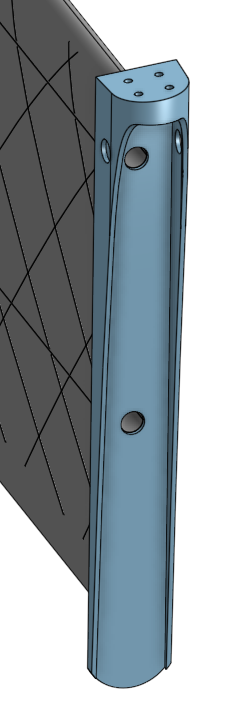
\includegraphics[height=0.4\linewidth]{figures/foot.png}
\caption{Wing endcap component serving as motor mount and landing foot. This multi-functional part closes the hollow wing structure, positions the motor ahead of the leading edge with a \(\pm\SI{5}{\degree}\) tilt for yaw control, and extends downward to protect the wing trailing edge during landing.}
\label{fig:wing_foot}
\end{figure}

\begin{figure}[htbp]
\centering
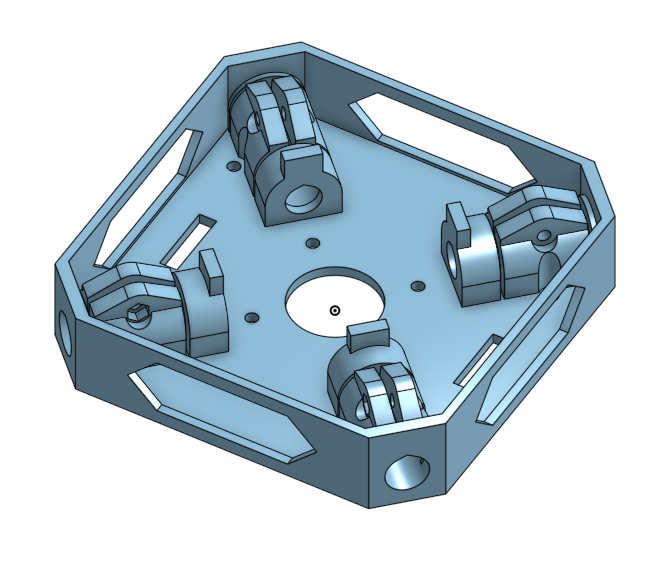
\includegraphics[width=0.6\linewidth]{figures/core.png}
\caption{Central core structure that clamps the carbon fiber spars. Two identical cores are used for ease of manufacturing: one houses the ESC, flight controller, and batteries (top), while the other serves as a structural clamp for the lower spars (bottom). A snap-on lid (not shown) covers the top core for additional stiffness and battery mounting.}
\label{fig:core_structure}
\end{figure}

\subsection{Wing Aerodynamics}

The aerodynamic surfaces were designed for efficient lift generation in the cruise speed range of \SIrange{5}{15}{\meter\per\second}.  
At a nominal flight velocity of \SI{10}{\meter\per\second} and chord length of \SI{0.25}{\meter}, the expected Reynolds number is on the order of \(1\times10^5\)–\(2\times10^5\), placing the operation in the low-Reynolds transitional regime.

The Reynolds number characterizes the ratio of inertial to viscous forces and is computed as
\begin{equation}
Re = \frac{\rho V c}{\mu} = \frac{V c}{\nu},
\label{eq:reynolds_number}
\end{equation}
where \(\rho\) is the air density, \(V\) is the airspeed, \(c\) is the chord length, \(\mu\) is the dynamic viscosity, and \(\nu\) is the kinematic viscosity of air.
Using standard atmospheric conditions at sea level (\(\rho = 1.225~\mathrm{kg/m^3}\), \(\nu = 1.4207 \times 10^{-5}~\mathrm{m^2/s}\)) and the wing chord length of \(c = 0.25~\mathrm{m}\), the Reynolds number is approximately \(Re \approx 1.76 \times 10^5\) at \SI{10}{\meter\per\second} and \(Re \approx 5.27 \times 10^5\) at \SI{30}{\meter\per\second}.

At the \SI{10}{\meter\per\second} cruise condition (\(Re \approx 2 \times 10^5\)), the NACA~0015 profile achieves a lift coefficient of approximately \(C_L \approx 0.97\) at \(\alpha \approx 10^\circ\) and a drag coefficient of \(C_D \approx 0.025\).
The target angle of attack in steady cruise was set to around \SI{10}{\degree}.  
At this design cruise angle of attack, the airfoil provides sufficient lift to support the vehicle weight at moderate forward speeds.
A detailed comparison of the NACA~0015 baseline airfoil against an improved AG25 airfoil, including aerodynamic performance metrics and their correlation with flight test results, is presented in Chapter~\ref{chapter:experiments-evaluation}.

Lift and drag forces were estimated using the analytical model introduced earlier,
\[
L = \tfrac{1}{2} \rho S C_L(\alpha) \|v_a\|^2, \quad
D = \tfrac{1}{2} \rho S C_D(\alpha) \|v_a\|^2,
\]
with \(\rho\) denoting air density, \(S\) the total projected wing area, and \(v_a\) the airspeed relative to the body.  
These analytical estimates guided the sizing of the vehicle and the placement of the aerodynamic surfaces relative to the center of gravity.

\paragraph{Quantitative estimate at \(12~\mathrm{m/s}\).}
Using \(\rho=1.225~\mathrm{kg/m^3}\), total projected wing area \(S \approx 0.318~\mathrm{m^2}\), \(C_L \approx 0.97\) at \(\alpha \approx 10^\circ\), and \(C_D \approx 0.025\), we obtain
\[
L \;=\; \tfrac{1}{2}\,\rho\,S\,C_L\,V^2
\;\approx\; \tfrac{1}{2}\cdot 1.225 \cdot 0.318 \cdot 0.97 \cdot (12)^2
\;\approx\; 27.2~\mathrm{N},
\]
\[
D \;=\; \tfrac{1}{2}\,\rho\,S\,C_D\,V^2
\;\approx\; \tfrac{1}{2}\cdot 1.225 \cdot 0.318 \cdot 0.025 \cdot (12)^2
\;\approx\; 0.70~\mathrm{N}.
\]
For the \SI{2.5}{kg} platform (\(W \approx 24.53~\mathrm{N}\)), the wings supply \(\approx 111\%\) of the weight at \(12~\mathrm{m/s}\), meaning the rotors can reduce thrust significantly and primarily need to overcome aerodynamic drag and provide control authority. The wing-induced drag corresponds to \(\approx 8.4~\mathrm{W}\) of propulsive power at \(12~\mathrm{m/s}\) (\(P_D = D\,V\)), not accounting for additional parasite/induced drag from the fuselage, rotors, and interference effects. These values are first-order estimates based on XFLR5 analysis and neglect propeller–wing interaction; they nonetheless quantify the expected forward-flight relief on rotor-induced power.

Propeller–wing interaction effects were not explicitly studied in this work.  
Since the wings are aligned with the rotor arms, partial overlap between the propeller wake and wing surface occurs, but its contribution to performance is assumed to be secondary compared to the main aerodynamic lift of the forward wings.  
Future investigations could employ CFD or wind-tunnel testing to quantify this coupling.

\subsection{Propulsion and Actuation}

The propulsion system was designed to maintain high agility while achieving efficient cruise performance.  
A thrust-to-weight ratio exceeding 3 was selected as a design target, enabling the vehicle to perform aggressive maneuvers and sustain up to \SI{3}{g} lateral acceleration, consistent with agility metrics reported in the multirotor literature.  
To meet this target, high-response racing-grade components were chosen:  
T-MOTOR VELOX~V2808 motors combined with HQProp~7×3.5×3 three-blade propellers.  
The resulting hover throttle is approximately 30\%, leaving sufficient control margin for disturbance rejection and attitude stabilization.

Motor and propeller performance were characterized experimentally to obtain both thrust and torque mappings.  
The measurements were performed using a single motor mounted on a six-axis force–torque sensor, with forces and torques recorded over a range of command inputs.  
The empirical relations between motor command, thrust, and torque were used to map the controller outputs into corresponding DShot commands for the flight controller.  
These mappings also served to estimate instantaneous energy consumption and mechanical efficiency during flight trials.

The motors are tilted outward by \SI{5}{\degree} to increase effective yaw torque authority.  
In the control model, this tilt is represented as a small rotation of the individual thrust vectors, effectively increasing the available moment around the vertical axis.  
No DShot timing modifications were required, and no direct RPM feedback control was implemented.  
Instead, the INDI controller integrates motor speed responses and compensates for small deviations, ensuring smooth dynamic performance.

Although the addition of wings increases the total inertia of the platform, particularly in yaw, the resulting damping improved stability and reduced sensitivity to high-frequency disturbances.  
No significant cross-coupling between roll and pitch dynamics was observed.  
Overall, the X-wing configuration provides a good compromise between efficiency and agility, maintaining the control simplicity of a quadrotor while offering measurable lift benefits in forward flight.  
Performance gains were compared analytically against a non-winged reference quadrotor of comparable size and propulsion, confirming a theoretical reduction in power consumption at moderate forward velocities.

% TODO: Add figure
% \begin{figure}[h]
% \centering
% \includegraphics[width=0.8\linewidth]{figures/xwing_layout.pdf}
% \caption{X-wing aerodynamic surface-enhanced quadrotor layout showing the symmetric dihedral configuration and component arrangement.}
% \label{fig:xwing_layout}
% \end{figure}

% !TeX root = ../main.tex

\chapter{Control Architecture}\label{chapter:control-architecture}

This chapter presents the flight control system used on the X-wing quadrotor.
The architecture combines (i) \emph{flatness-based reference generation} for dynamically
feasible trajectories, (ii) a \emph{geometric outer loop} on $SE(3)$ that turns
translational tracking errors into desired attitude and collective thrust, and
(iii) an \emph{Incremental Nonlinear Dynamic Inversion (INDI)} inner loop that
realizes the requested angular dynamics while rejecting unmodeled aerodynamic
effects from the wings.
The wings are \emph{not} explicitly modeled in the controller; instead, their influence
is treated as a disturbance and compensated incrementally by INDI
\cite{Smeur2016,Oosedo2017,vanKampen2018,Tzoumanikas2021}.

\section{Reference Generation}\label{sec:ref-gen}
Quadrotor dynamics are differentially flat with respect to
$\mathbf{p}_d=[x_d,y_d,z_d]^\top$ and $\psi_d$.
We generate $(\mathbf{p}_d,\dot{\mathbf{p}}_d,\ddot{\mathbf{p}}_d,\psi_d)$
from a minimum-snap polynomial or flatness-based planner; jerk/snap may be used internally
for smoothness but are not required by the controller interface.

\paragraph{Coordinated-turn option.}
In forward flight, sideslip can be bounded by aligning the body $x$-axis with the
horizontal velocity and setting a yaw-rate reference approximately as
\begin{equation}
\dot{\psi}_d \;\approx\; \frac{a_{y,d}}{V_d\cos\theta_d},
\end{equation}
where $a_{y,d}$ is the desired lateral acceleration, $V_d=\|\dot{\mathbf{p}}_d\|$, and
$\theta_d$ the pitch. We use this option when tracking fast, curving
trajectories; otherwise $\psi_d$ follows a commanded heading.

\section{Geometric Outer Loop}\label{sec:outer}
The outer loop maps position/velocity errors to a desired attitude $R_d\in SO(3)$
and a collective thrust $f_{\text{coll}}$.

\subsection{Translational feedback and force target}\label{sec:outer-force}
Let $\tilde{\mathbf{p}}=\mathbf{p}_d-\mathbf{p}$ and $\tilde{\mathbf{v}}=\dot{\mathbf{p}}_d-\mathbf{v}$.
With diagonal gains $\mathbf{k}_p,\mathbf{k}_v>0$ (elementwise),
\begin{equation}
\mathbf{a}_c \;=\; \mathbf{k}_p\odot\tilde{\mathbf{p}}
                  \;+\; \mathbf{k}_v\odot\tilde{\mathbf{v}}
                  \;+\; \ddot{\mathbf{p}}_d \;-\; \mathbf{g},
\label{eq:ac-nom}
\end{equation}
defines the nominal commanded acceleration in the world frame (ENU, $\mathbf{g}=[0,0,-g]^\top$).

\paragraph{Aerodynamic feedforward from onboard sensing.}
We estimate a body-frame specific force $\mathbf{a}_B$ from the IMU (bias-compensated)
or a model fallback and low-pass filter it, $\mathbf{a}_{B,f}=\mathrm{LPF}_a(\mathbf{a}_B)$.
From filtered motor speeds $\boldsymbol{\omega}_m$ we form
$\mathbf{f}_f = k_t\,\mathrm{LPF}_m(\boldsymbol{\omega}_m^{\circ 2})+\mathbf{b}$,
so that $f_{T,f}=\mathbf{1}^\top\mathbf{f}_f$.
A world-frame aero-compensation term follows as
\begin{equation}
\mathbf{a}_{\text{aero}} \;=\; R\!\left(\frac{f_{T,f}}{m}\,\mathbf{e}_3 - \mathbf{a}_{B,f}\right),
\qquad
\mathbf{a}_c \;\leftarrow\; \mathbf{a}_c + \mathbf{a}_{\text{aero}}
\;\;\text{if } z>0.5~\mathrm{m}.
\label{eq:aero-comp-outer}
\end{equation}
Intuitively, $R(f_{T,f}\mathbf{e}_3/m)$ is the thrust-induced specific force in the world;
subtracting the measured specific force yields the unmodeled aero contribution to be
fed forward.

\subsection{Attitude target and thrust projection}\label{sec:outer-att}
We set the desired body $z$-axis to the direction of the commanded acceleration,
$\mathbf{z}_B^d=\mathbf{a}_c/\|\mathbf{a}_c\|$.
For heading, we prefer a coordinated-turn alignment:
\[
\mathbf{x}_c =
\begin{cases}
\dot{\mathbf{p}}_d/\|\dot{\mathbf{p}}_d\|, & \|\dot{\mathbf{p}}_d\|>0.2~\mathrm{m/s},\\
R_z(\psi_d)\,\mathbf{e}_x, & \text{otherwise},
\end{cases}
\quad (\mathbf{x}_c)_z=0,\;\|\mathbf{x}_c\|=1.
\]
To avoid the degeneracy $\mathbf{z}_B^d\parallel\mathbf{x}_c$, we set
$\mathbf{x}_c\leftarrow -\mathbf{e}_z$ if $\angle(\mathbf{z}_B^d,\mathbf{x}_c)<5^\circ$.
Then
\begin{equation}
\mathbf{y}_B^d = \frac{\mathbf{z}_B^d\times\mathbf{x}_c}{\|\mathbf{z}_B^d\times\mathbf{x}_c\|},
\qquad
\text{flip } \mathbf{y}_B^d \text{ if } (\mathbf{y}_B^d)^\top(R\mathbf{e}_y)<0,
\qquad
\mathbf{x}_B^d = \frac{\mathbf{y}_B^d\times\mathbf{z}_B^d}{\|\mathbf{y}_B^d\times\mathbf{z}_B^d\|},
\end{equation}
and $R_d=[\,\mathbf{x}_B^d\;\mathbf{y}_B^d\;\mathbf{z}_B^d\,]$.
We compute collective thrust by projection to reduce transients:
\begin{equation}
f_{\text{coll}} \;=\; m\,\mathbf{a}_c^\top (R\mathbf{e}_3).
\label{eq:thrust-proj}
\end{equation}

\subsection{Tilt-prioritized attitude control and rate reference}\label{sec:tilt-prio}
Following the tilt-prioritized design of Föhn (2020), with attitude error
$q_e=q^{-1}\!\otimes q_d$ and gains $k_{\text{att},xy},k_{\text{att},z}$,
\begin{align}
T_{\text{att}} &= \mathrm{diag}(k_{\text{att},xy},k_{\text{att},xy},k_{\text{att},z}),
\\
\mathbf{t}(q_e) &= 
\begin{bmatrix}
q_{e,w}q_{e,x}-q_{e,y}q_{e,z}\\
q_{e,w}q_{e,y}+q_{e,x}q_{e,z}\\
q_{e,z}
\end{bmatrix},
\quad \text{if } q_{e,w}\le 0 \text{ then } t_3\leftarrow -t_3,
\\
\boldsymbol{\omega}_d &= \frac{2}{\sqrt{q_{e,w}^2+q_{e,z}^2}}\;T_{\text{att}}\;\mathbf{t}(q_e).
\label{eq:omega-d}
\end{align}
A simple rate-plus-error form produces an \emph{angular-acceleration proxy}
for INDI:
\begin{equation}
\boldsymbol{\alpha}_d \;=\; \boldsymbol{\omega}_d \;+\; 
\mathbf{k}_{\text{rate}}\odot(\boldsymbol{\omega}_d-\boldsymbol{\omega}).
\label{eq:alpha-d}
\end{equation}
We forward $(R_d,f_{\text{coll}},\boldsymbol{\alpha}_d)$ to the inner loop.

\section{INDI Inner Loop}\label{sec:indi}
The inner loop realizes the requested rotational dynamics robustly without an explicit
aerodynamic model. Over a small sampling interval $\Delta t$, the change in the measured
output $\mathbf{y}$ (specific force or angular acceleration proxy) satisfies
\begin{equation}
\Delta\mathbf{y} \;\approx\; B\,\Delta\mathbf{u},
\end{equation}
with $B$ the (local) control-effectiveness matrix and $\Delta\mathbf{d}$ (disturbance change)
second order in $\Delta t$; hence the incremental update largely cancels unmodeled
aerodynamics \cite{Smeur2016,Oosedo2017,vanKampen2018,Tzoumanikas2021}.

\subsection{Measured/filtered quantities}\label{sec:indi-sensed}
We use gyroscope rates $\boldsymbol{\omega}$ and their filtered derivative as an acceleration proxy,
\begin{equation}
\dot{\boldsymbol{\omega}}_f \;=\; \frac{\mathrm{d}}{\mathrm{d}t}\big(\mathrm{LPF}_\omega(\boldsymbol{\omega})\big),
\end{equation}
and reconstruct filtered rotor thrusts from motor speeds as in \eqref{eq:aero-comp-outer}. The
filtered rotor moments follow from the allocation matrix $G$:
\begin{equation}
\begin{bmatrix} f_{T,f}\\ \boldsymbol{\tau}_f \end{bmatrix} \;=\; G\,\mathbf{f}_f.
\label{eq:tau-f}
\end{equation}

\subsection{Nominal NDI versus incremental INDI moments}\label{sec:ndi-vs-indi}
Let $\boldsymbol{\mu}=[\mu_0,\mu_x,\mu_y,\mu_z]^\top=[f_T,\tau_x,\tau_y,\tau_z]^\top$.
We form two moment requests:
\begin{align}
\boldsymbol{\mu}_{\text{NDI}} &=
\begin{bmatrix}
m\,f_{\text{coll}}\\
(J\boldsymbol{\alpha}_d + \boldsymbol{\omega}\times J\boldsymbol{\omega})_x\\
(J\boldsymbol{\alpha}_d + \boldsymbol{\omega}\times J\boldsymbol{\omega})_y\\
(J\boldsymbol{\alpha}_d + \boldsymbol{\omega}\times J\boldsymbol{\omega})_z
\end{bmatrix},
\label{eq:mu-ndi}\\
\boldsymbol{\mu}_{\text{INDI}} &=
\begin{bmatrix}
m\,f_{\text{coll}}\\
\boldsymbol{\tau}_f + J\big(\boldsymbol{\alpha}_d - \dot{\boldsymbol{\omega}}_f\big)
\end{bmatrix}.
\label{eq:mu-indi}
\end{align}
Equation~\eqref{eq:mu-indi} is the incremental update: the moment change uses the mismatch
between desired and measured angular accelerations, injecting the \emph{measured} effectiveness
$J$ and $\boldsymbol{\tau}_f$.

\paragraph{Yaw-stability tweak.}
To avoid yaw oscillations observed in practice, we blend the two requests and set
\begin{equation}
\mu_z \;\leftarrow\; (\boldsymbol{\mu}_{\text{NDI}})_z,
\end{equation}
while keeping roll/pitch from \eqref{eq:mu-indi}.

\paragraph{Mode switch at low altitude.}
For takeoff and near-ground operation we disable INDI and use
$\boldsymbol{\mu}\leftarrow\boldsymbol{\mu}_{\text{NDI}}$ if $z<0.5$~m or a configuration flag is off.

\subsection{Update to rotor thrusts}\label{sec:indi-to-rotors}
With the inverse allocation matrix $G^{-1}$ (precomputed from geometry, including motor tilt),
the commanded rotor thrusts are
\begin{equation}
\mathbf{u} \;=\; G^{-1}\,\boldsymbol{\mu},
\qquad f_T=\mathbf{1}^\top\mathbf{u}.
\label{eq:indi-allocation}
\end{equation}
Each rotor thrust maps to speed via the quadratic thrust curve,
\begin{equation}
f_i \;=\; k_t\,\omega_i^2 \;+\; b_i,
\qquad
\omega_i \;=\; \sqrt{\max(0,(f_i-b_i)/k_t)}.
\label{eq:thrust-map}
\end{equation}
Commands are sent to the ESCs (DShot). Saturation and safety guards are applied at the actuation layer.

\section{Control Allocation and Constraints}\label{sec:allocation}
The allocation matrix $G\in\mathbb{R}^{4\times 4}$ maps individual rotor thrusts to total thrust
and body moments,
\begin{equation}
\boldsymbol{\mu}=G\,\mathbf{u},
\qquad
\mathbf{u}=[f_1,f_2,f_3,f_4]^\top,
\end{equation}
and encodes the arm geometry and $\SI{5}{\degree}$ motor tilt (see Chapter~\ref{chapter:experimental-setup}).
We use its inverse for real-time mapping \eqref{eq:indi-allocation}.
Commanded thrusts are clipped to $f_i\in[f_{\min},f_{\max}]$ and total thrust is bounded for hardware safety.
(When needed, a constrained least-squares allocator can replace $G^{-1}$ to enforce non-negativity and torque bounds.)

\section{Implementation Notes}\label{sec:impl-notes}
\paragraph{Filtering.}
First-order low-pass filters $\mathrm{LPF}_a,\mathrm{LPF}_\omega,\mathrm{LPF}_m$ use cutoffs
chosen below the control bandwidth to avoid amplifying sensor noise in $\dot{\boldsymbol{\omega}}_f$.
All filters are tuned consistently across the outer/inner loops.

\paragraph{Sensing and fusion.}
The controller runs with IMU rates at high frequency; position/velocity references come from Vicon or onboard state estimation.
Delays are kept small by using incremental updates; no explicit delay compensation was required.

\paragraph{Scheduling.}
The inner INDI loop runs faster than the outer geometric loop (rate separation).
Allocation and motor mapping execute at the inner-loop rate.

\paragraph{Logging and health.}
We log $\boldsymbol{\omega},\dot{\boldsymbol{\omega}}_f,\mathbf{f}_f,\boldsymbol{\tau}_f$ and the residual
$\boldsymbol{\tau}_f - J\dot{\boldsymbol{\omega}}_f - \boldsymbol{\omega}\times J\boldsymbol{\omega}$ to monitor effectiveness.
Guard checks reject invalid states or setpoints.

\section{Tuning Guidance}\label{sec:tuning}
\begin{itemize}
  \item \textbf{Outer loop} $\mathbf{k}_p,\mathbf{k}_v$: increase until overshoot appears in step tests, then back off; clip $\tilde{\mathbf{p}},\tilde{\mathbf{v}}$ to limit transients.
  \item \textbf{Attitude gains} $k_{\text{att},xy},k_{\text{att},z}$: prioritize $x$–$y$ for agility; keep $k_{\text{att},z}$ smaller to avoid yaw chatter.
  \item \textbf{Rate gains} $\mathbf{k}_{\text{rate}}$: start small; raise until $\dot{\boldsymbol{\omega}}_f$ tracks $\boldsymbol{\alpha}_d$ with minimal lag.
  \item \textbf{Filters}: set cutoffs so that $\dot{\boldsymbol{\omega}}_f$ is smooth but responsive; align motor-speed and accelerometer filter cutoffs.
  \item \textbf{Allocation}: verify $G$ from CAD (arm length, tilt, motor spin) and validate $G^{-1}$ via static torque tests.
\end{itemize}

\section{Summary}\label{sec:ctrl-summary}
The proposed control system stacks a geometric $SE(3)$ outer loop with an INDI inner loop.
The outer loop produces $(R_d,f_{\text{coll}},\boldsymbol{\alpha}_d)$ by combining
proportional–derivative translational feedback with an aero feedforward term from onboard sensing,
and a coordinated-turn attitude construction.
The INDI layer then incrementally inverts the rotational dynamics using measured effectiveness,
blending a nominal NDI yaw to suppress oscillations.
This architecture achieves robust tracking across hover and forward-flight regimes while compensating
for the unmodeled aerodynamic influence of the X-wing surfaces.

% --- References used in this chapter ---
% Add to your .bib if not already present:
% \cite{Smeur2016,Oosedo2017,vanKampen2018,Tzoumanikas2021}
% (Optionally add Föhn 2020 for tilt-prioritized attitude control.)


% !TeX root = ../main.tex

\chapter{Experimental Setup}\label{chapter:experimental-setup}

\section{Experimental Setup}
\label{sec:experimental_setup}

This section documents the hardware configuration, software stack, and test facilities that enabled the experimental evaluation of the aerodynamic surface-enhanced quadrotor. The setup was designed to be fully reproducible, with all control and estimation software running on open frameworks and all data recorded for subsequent analysis.

\subsection{Hardware}

\subsubsection{Airframe and Propulsion}
The experimental platform consists of an X-wing aerodynamic surface-enhanced quadrotor (Fig.~\ref{fig:xwing_platform}) with a total mass of \SI{2.5}{\kilogram} (without batteries: \SI{1.75}{\kilogram}). Each of the four T-MOTOR VELOX~V2808 motors produces a maximum static thrust of approximately \SI{22}{\newton}, resulting in a total available thrust of \SI{88}{\newton} and a thrust-to-weight ratio of 3.59 at nominal \SI{22.2}{\volt} (6S~LiPo). The propulsion system employs HQProp 7×3.5×3 three-blade racing propellers optimized for medium–high efficiency in the forward-flight regime.

The wings feature a NACA~0015 airfoil with a length of \SI{450}{\milli\meter} and a chord of \SI{250}{\milli\meter}. Four identical fixed wings are arranged orthogonally (\SI{90}{\degree} between adjacent wings) and mounted with alternating dihedral and anhedral angles of $\pm\SI{45}{\degree}$. The wings are attached to the central frame using two carbon spars (\SI{10}{\milli\meter} outer diameter) clamped into the core structure, allowing for fast removal. The center frame and motor mounts are 3D-printed from standard PLA, while the wing surfaces are printed from lightweight PLA~Aero. The total projected horizontal area of all wings is approximately $S_\mathrm{t} = 0.318~\si{\meter\squared}$.

Each motor is mounted with a \SI{5}{\degree} tilt to improve yaw authority. The center of gravity is located at the geometric center of the vehicle, aligned with the midpoint between all four motors, and approximately at one quarter of the wing chord length from the leading edge.

\begin{figure}[htbp]
\centering
\begin{tikzpicture}[scale=1.5]
    % Define motor positions (X configuration)
    \coordinate (M1) at (1.5, -1.5);  % Bottom right
    \coordinate (M2) at (1.5, 1.5);   % Top right
    \coordinate (M3) at (-1.5, -1.5); % Bottom left
    \coordinate (M4) at (-1.5, 1.5);  % Top left
    
    % Draw center cross (arms)
    \draw[very thick, gray!50] (-1.5, -1.5) -- (1.5, 1.5);
    \draw[very thick, gray!50] (-1.5, 1.5) -- (1.5, -1.5);
    
    % Draw motors as circles with rotation arrows
    % Motor 1 (Bottom Right) - CW - arrow below
    \draw[thick, fill=gray!20] (M1) circle (0.5cm);
    \node[font=\Large\bfseries] at (M1) {1};
    \draw[->, thick, TUMBlue, line width=1.5pt] (M1) ++(315:0.4cm) arc (315:225:0.4cm);
    
    % Motor 2 (Top Right) - CCW - arrow above
    \draw[thick, fill=gray!20] (M2) circle (0.5cm);
    \node[font=\Large\bfseries] at (M2) {2};
    \draw[->, thick, TUMBlue, line width=1.5pt] (M2) ++(45:0.4cm) arc (45:135:0.4cm);
    
    % Motor 3 (Bottom Left) - CCW - arrow below
    \draw[thick, fill=gray!20] (M3) circle (0.5cm);
    \node[font=\Large\bfseries] at (M3) {3};
    \draw[->, thick, TUMBlue, line width=1.5pt] (M3) ++(225:0.4cm) arc (225:315:0.4cm);
    
    % Motor 4 (Top Left) - CW - arrow above
    \draw[thick, fill=gray!20] (M4) circle (0.5cm);
    \node[font=\Large\bfseries] at (M4) {4};
    \draw[->, thick, TUMBlue, line width=1.5pt] (M4) ++(135:0.4cm) arc (135:45:0.4cm);
    
    % Forward direction arrow (pointing upward)
    \draw[->, very thick, red, line width=2pt] (0, 2.5) -- (0, 3.2);
    \node[red, font=\Large\bfseries] at (0, 3.6) {Forward};
    
\end{tikzpicture}
\caption{Motor configuration and numbering convention. Blue arrows indicate rotation direction (clockwise for motors 1 and 4, counter-clockwise for motors 2 and 3).}
\label{fig:motor_configuration}
\end{figure}

\begin{figure}[htbp]
\centering
\begin{minipage}[b]{0.48\textwidth}
    \centering
    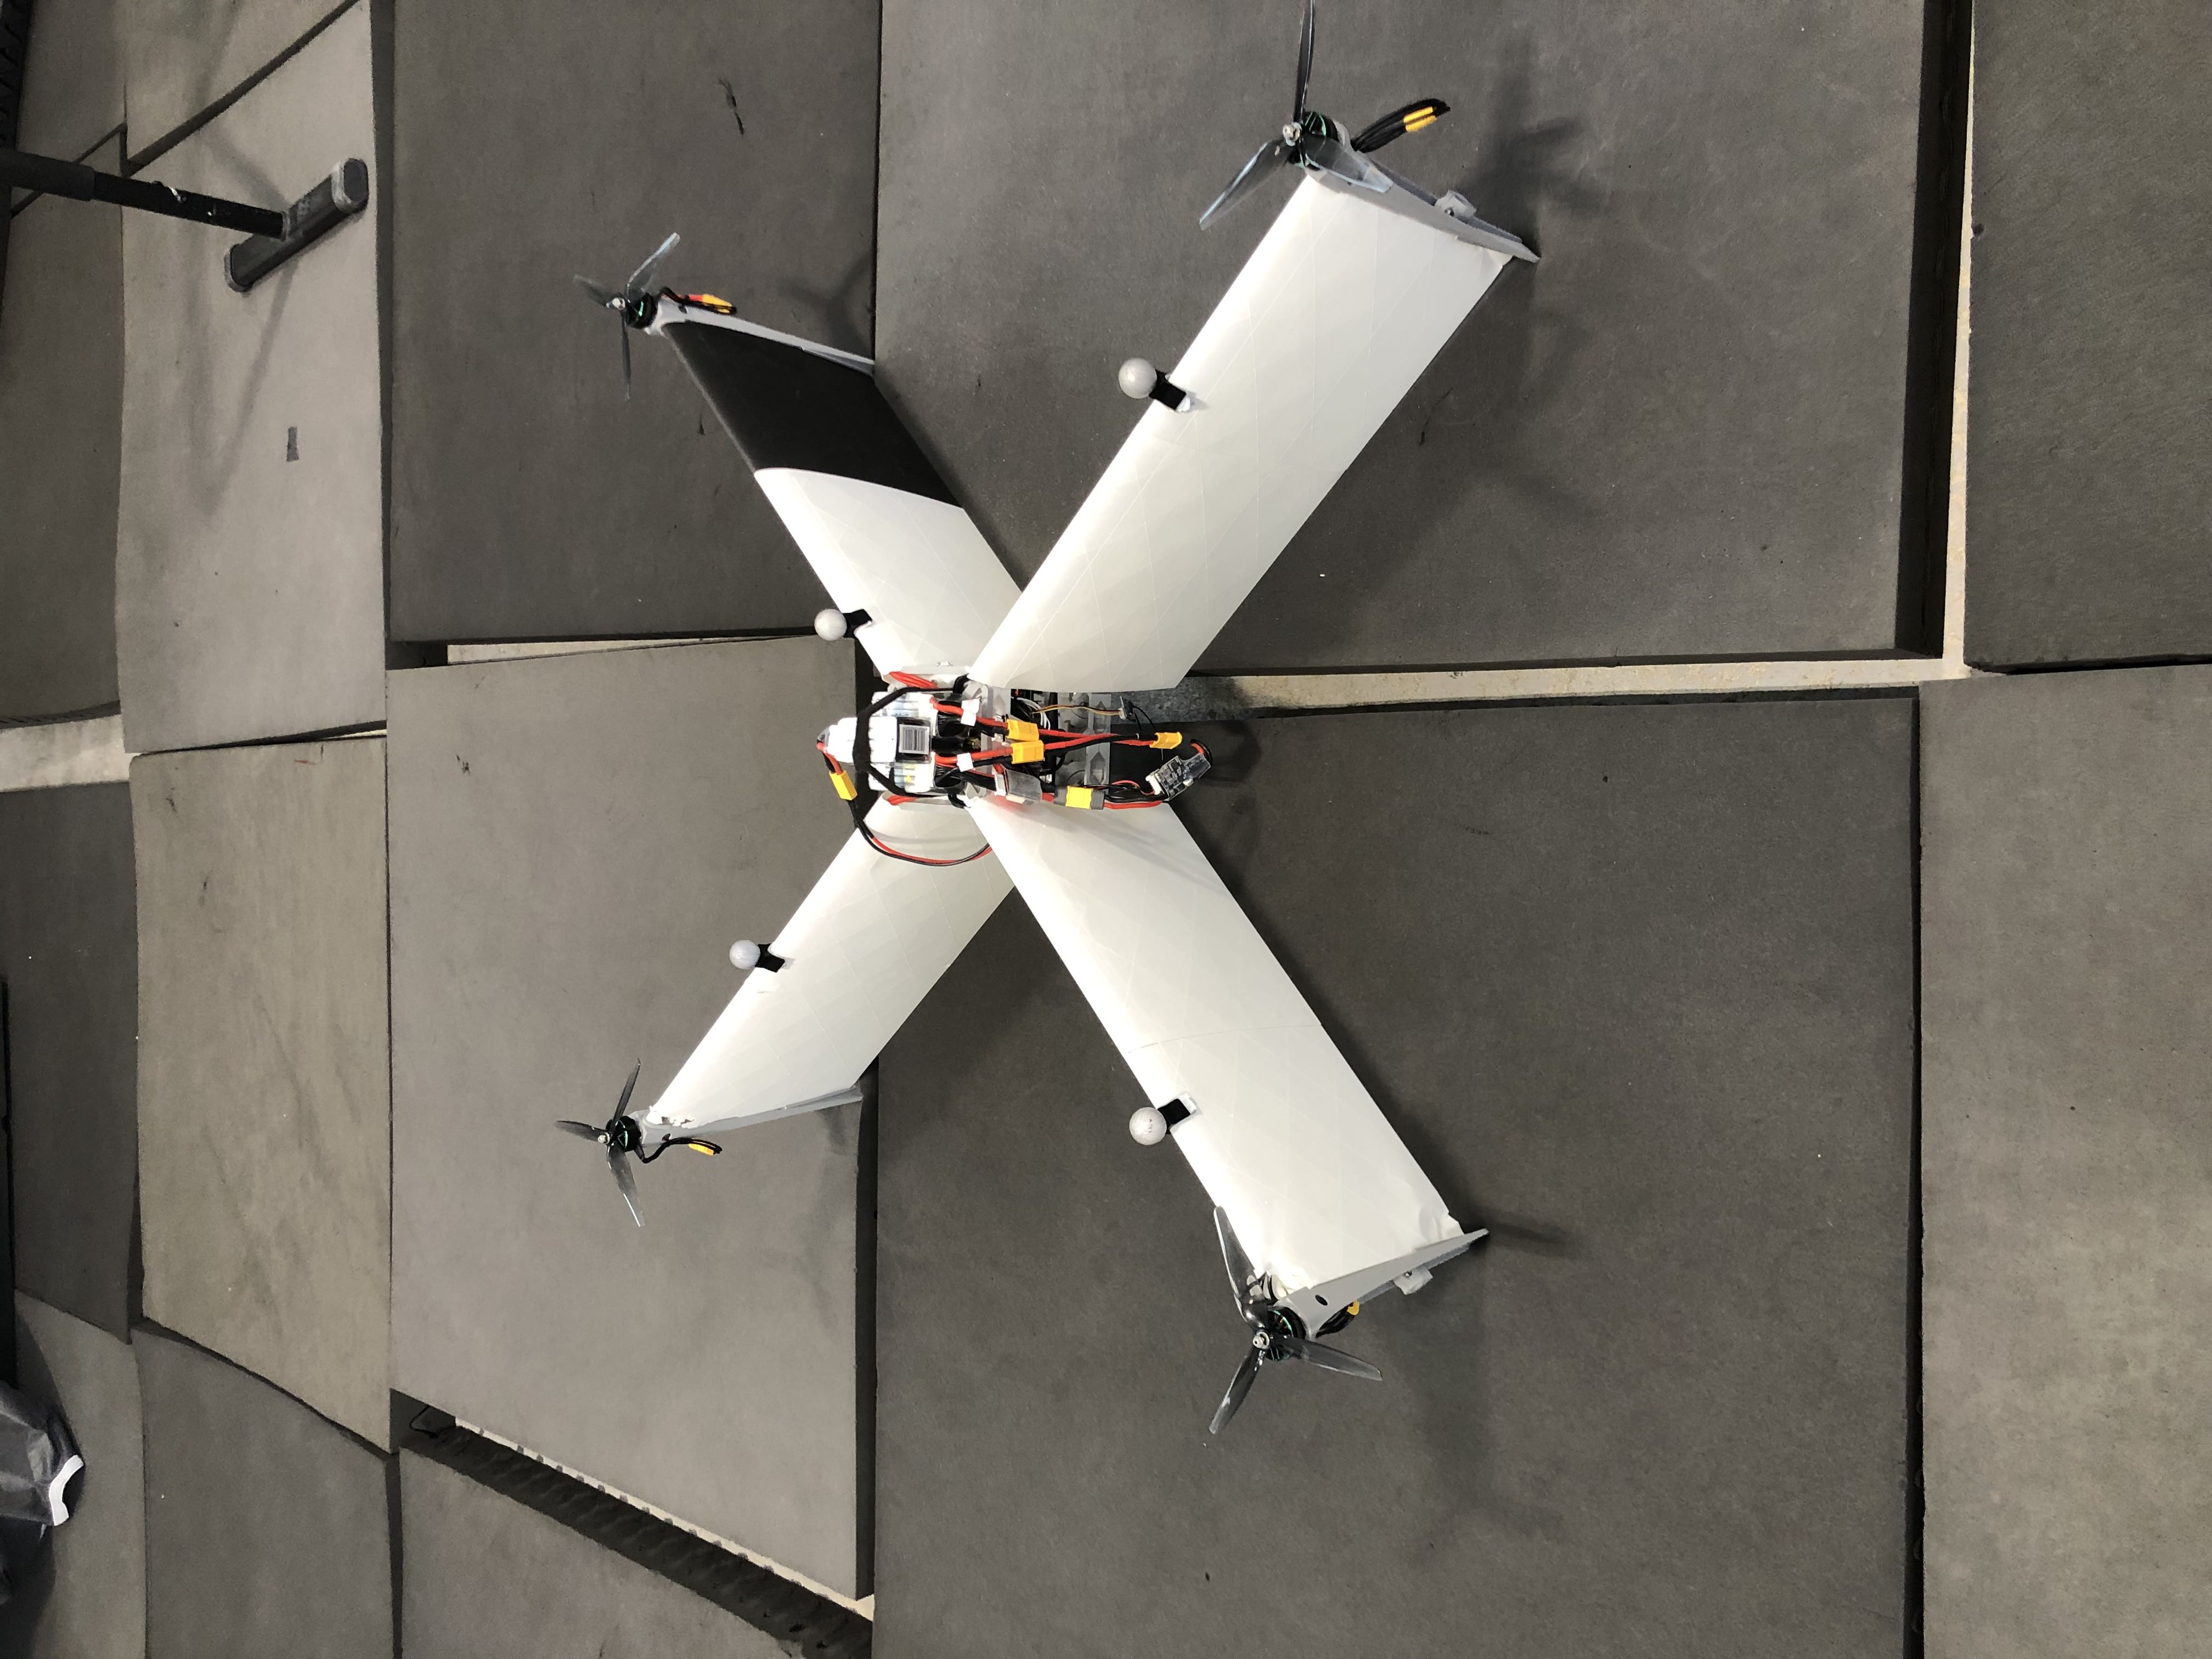
\includegraphics[width=\textwidth,angle=-90]{figures/drone_hover.jpg}
    \caption*{(a) Top view showing X-wing configuration with orthogonal wing arrangement.}
\end{minipage}
\hfill
\begin{minipage}[b]{0.48\textwidth}
    \centering
    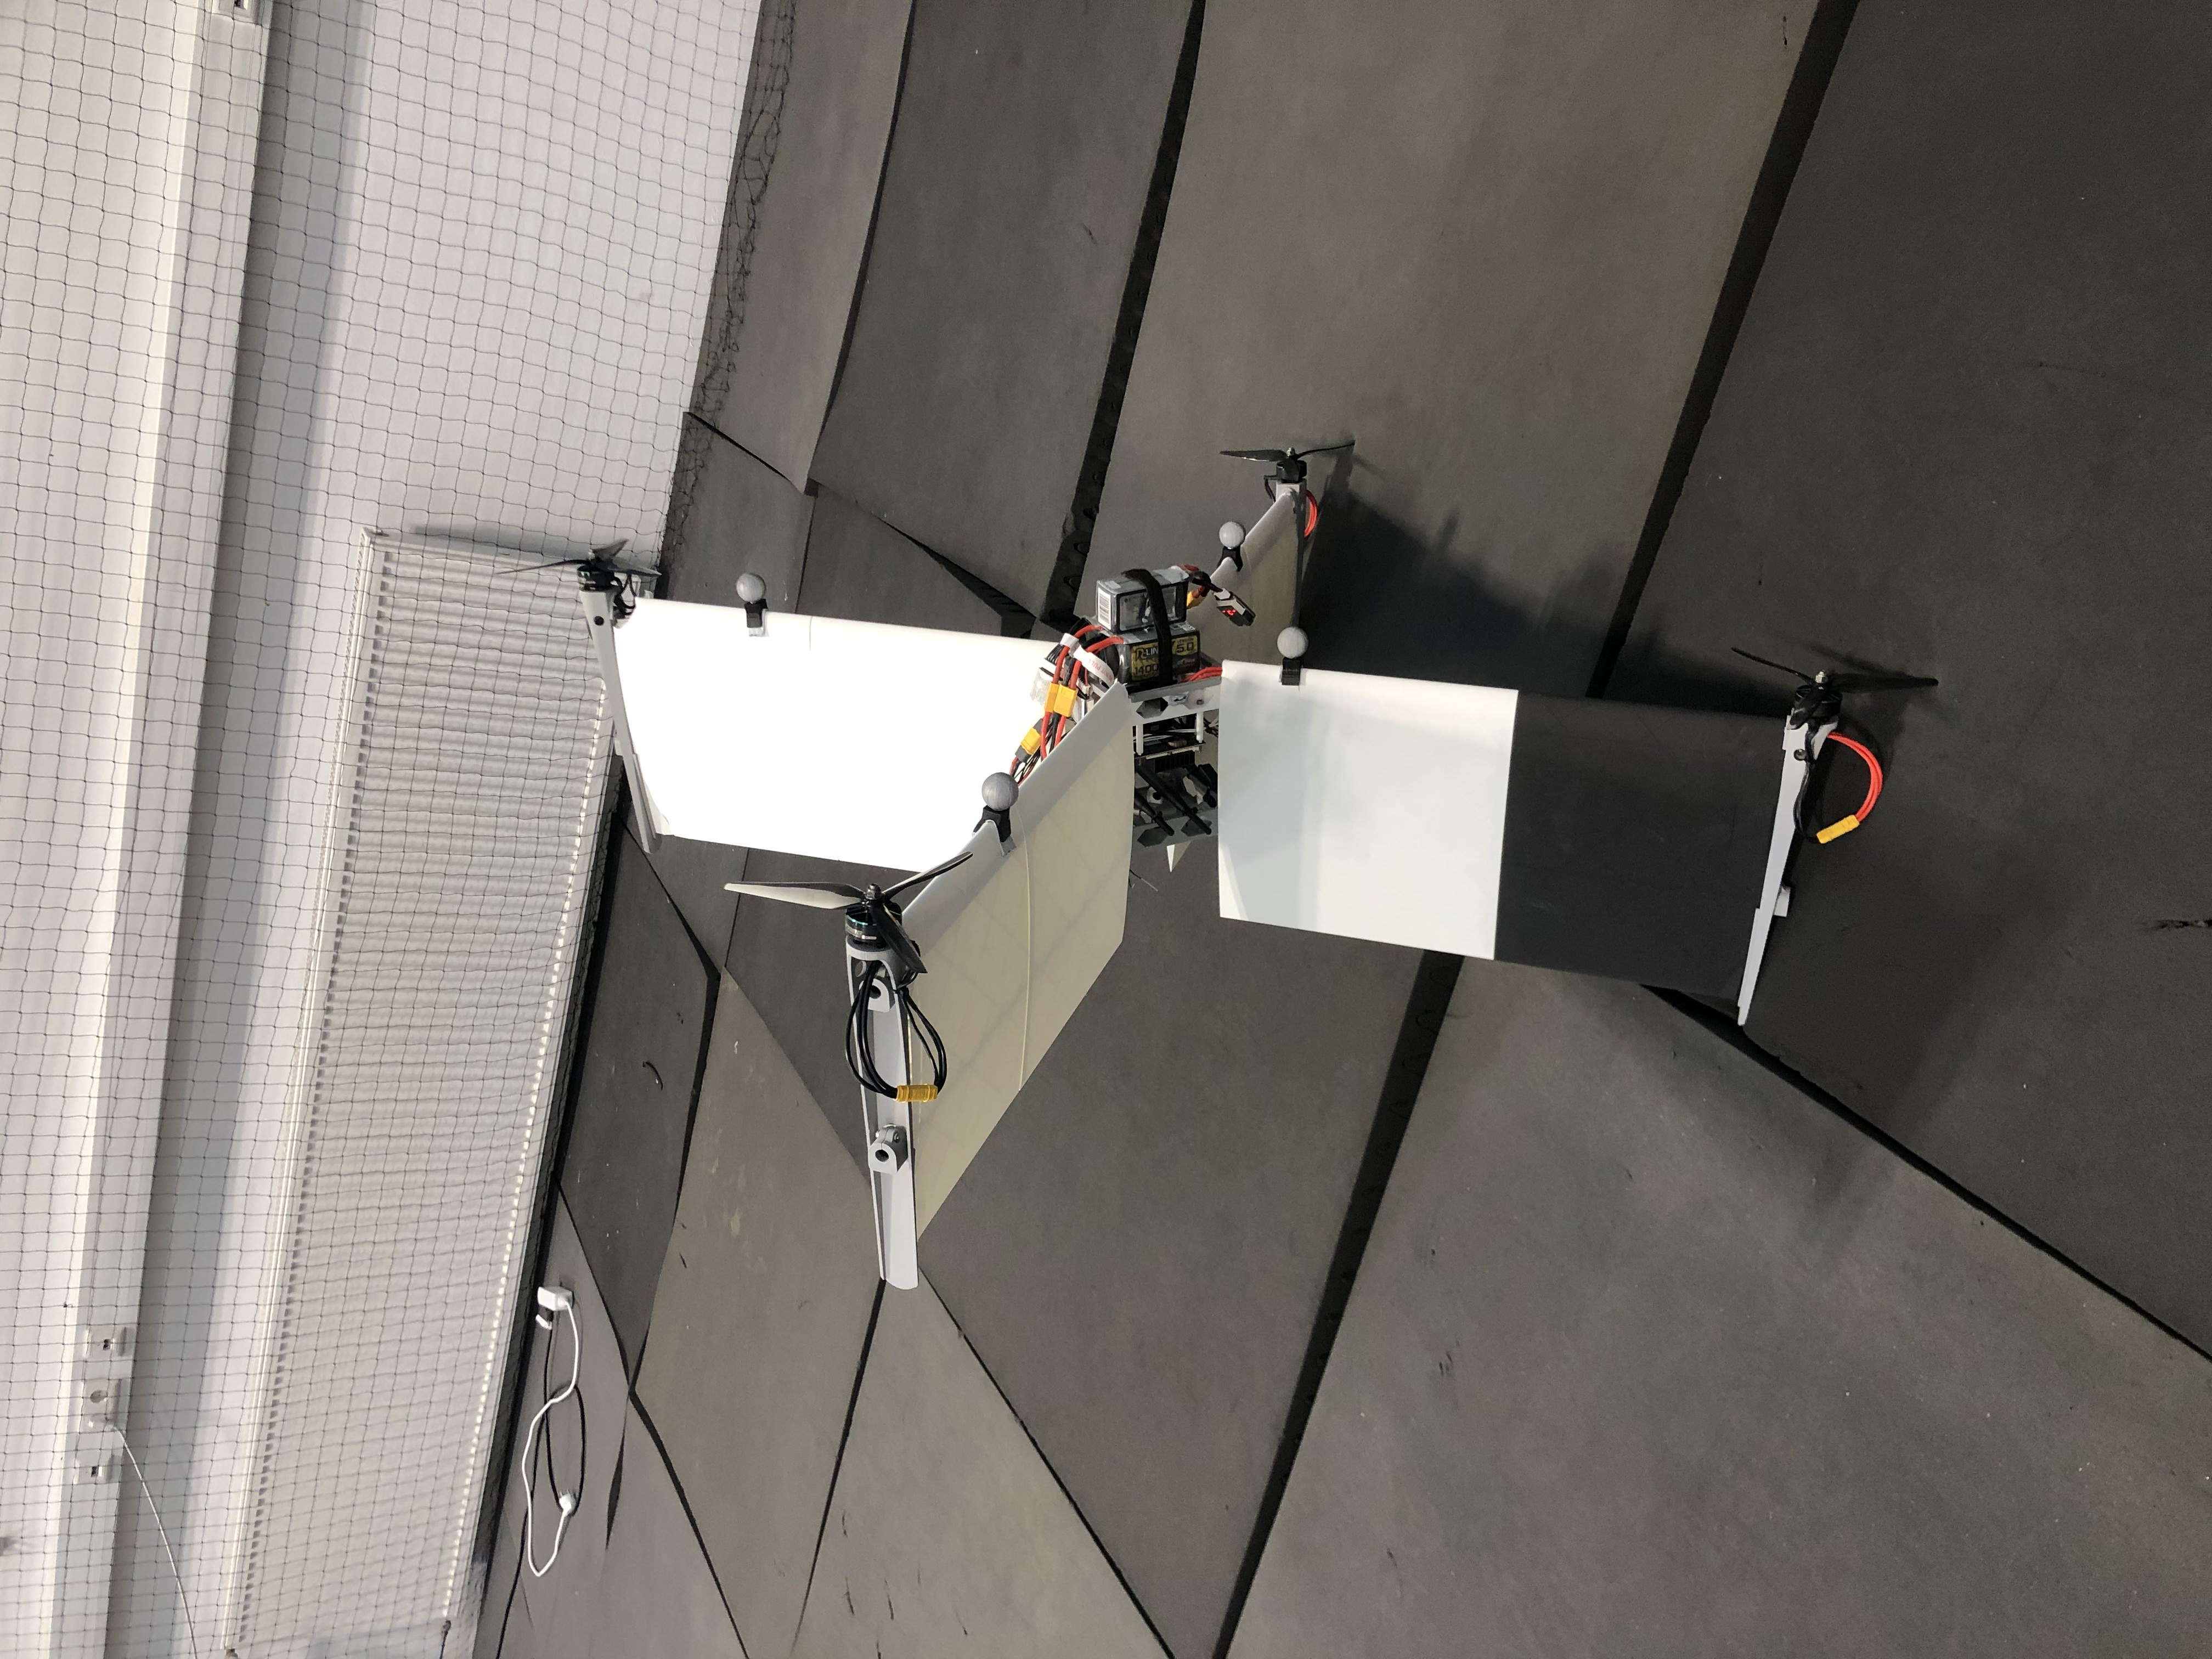
\includegraphics[width=\textwidth,angle=-90]{figures/drone_wing_flight.jpg}
    \caption*{(b) Side view showing forward flight orientation.}
\end{minipage}
\caption{The experimental X-wing aerodynamic surface-enhanced quadrotor platform.}
\label{fig:xwing_platform}
\end{figure}

\subsubsection{Platform Variants}
Two variants of the X-wing platform were used for efficiency experiments. The baseline platform (described above and shown in Fig.~\ref{fig:xwing_platform}) served as the primary testbed for control development and initial efficiency characterization. 

An improved variant with modified aerodynamic characteristics was developed by [Colleague Name]\footnote{[Colleague Full Name], Bachelor thesis, [Lab Name], [Year]. The improved design builds upon the baseline platform and incorporates aerodynamic refinements.} and employed for comparative efficiency measurements. The improved variant features a different airfoil profile and modified dihedral angles optimized for enhanced lift-to-drag performance in forward flight. All other subsystems—propulsion, avionics, mass, and control architecture—remain identical between both platforms, allowing for direct aerodynamic comparison.

Table~\ref{tab:platform_comparison} summarizes the key differences between the two variants.

\begin{table}[h]
\centering
\caption{Comparison of baseline and improved X-wing platform variants.}
\label{tab:platform_comparison}
\small
\begin{tabularx}{\textwidth}{lXX}
\toprule
Parameter & Baseline Platform & Improved Platform \\
\midrule
Airfoil & NACA~0015 & ag25 \\
Dihedral/Anhedral & $\pm\SI{45}{\degree}$ (alternating) & $\pm\SI{20}{\degree}$ (alternating) \\
Wing Length & \SI{450}{\milli\meter} & \SI{500}{\milli\meter} \\
Wing Chord & \SI{250}{\milli\meter} & \SI{230}{\milli\meter} \\
Motor Tilt (Yaw Authority) & $\pm\SI{5}{\degree}$ & $\pm\SI{5}{\degree}$ \\
Total Mass & \SI{2.5}{\kilogram} & \SI{2.2}{\kilogram} \\
Propulsion & T-MOTOR VELOX~V2808 + HQProp 7×3.5×3 & Identical \\
Avionics & Kakute~H7 + Jetson Orin Nano & Identical \\
\bottomrule
\end{tabularx}
\end{table}

\subsubsection{Thrust Characterization and Command Mapping}
To accurately relate motor command inputs to generated thrust, a static thrust characterization was performed for the chosen motor–propeller configuration.  
A single T-MOTOR~VELOX~V2808 motor equipped with an HQProp~7×3.5×3 propeller was mounted on a six-axis force–torque sensor (Rokubi~Mini) using a custom 3D-printed fixture.  
The setup allowed precise measurement of the vertical force while commanding the motor through the same DShot interface used in flight (Fig.~\ref{fig:force_test_stand}).

\begin{figure}[h]
\centering
\begin{tikzpicture}
\node[anchor=south west,inner sep=0] (image) at (0,0) {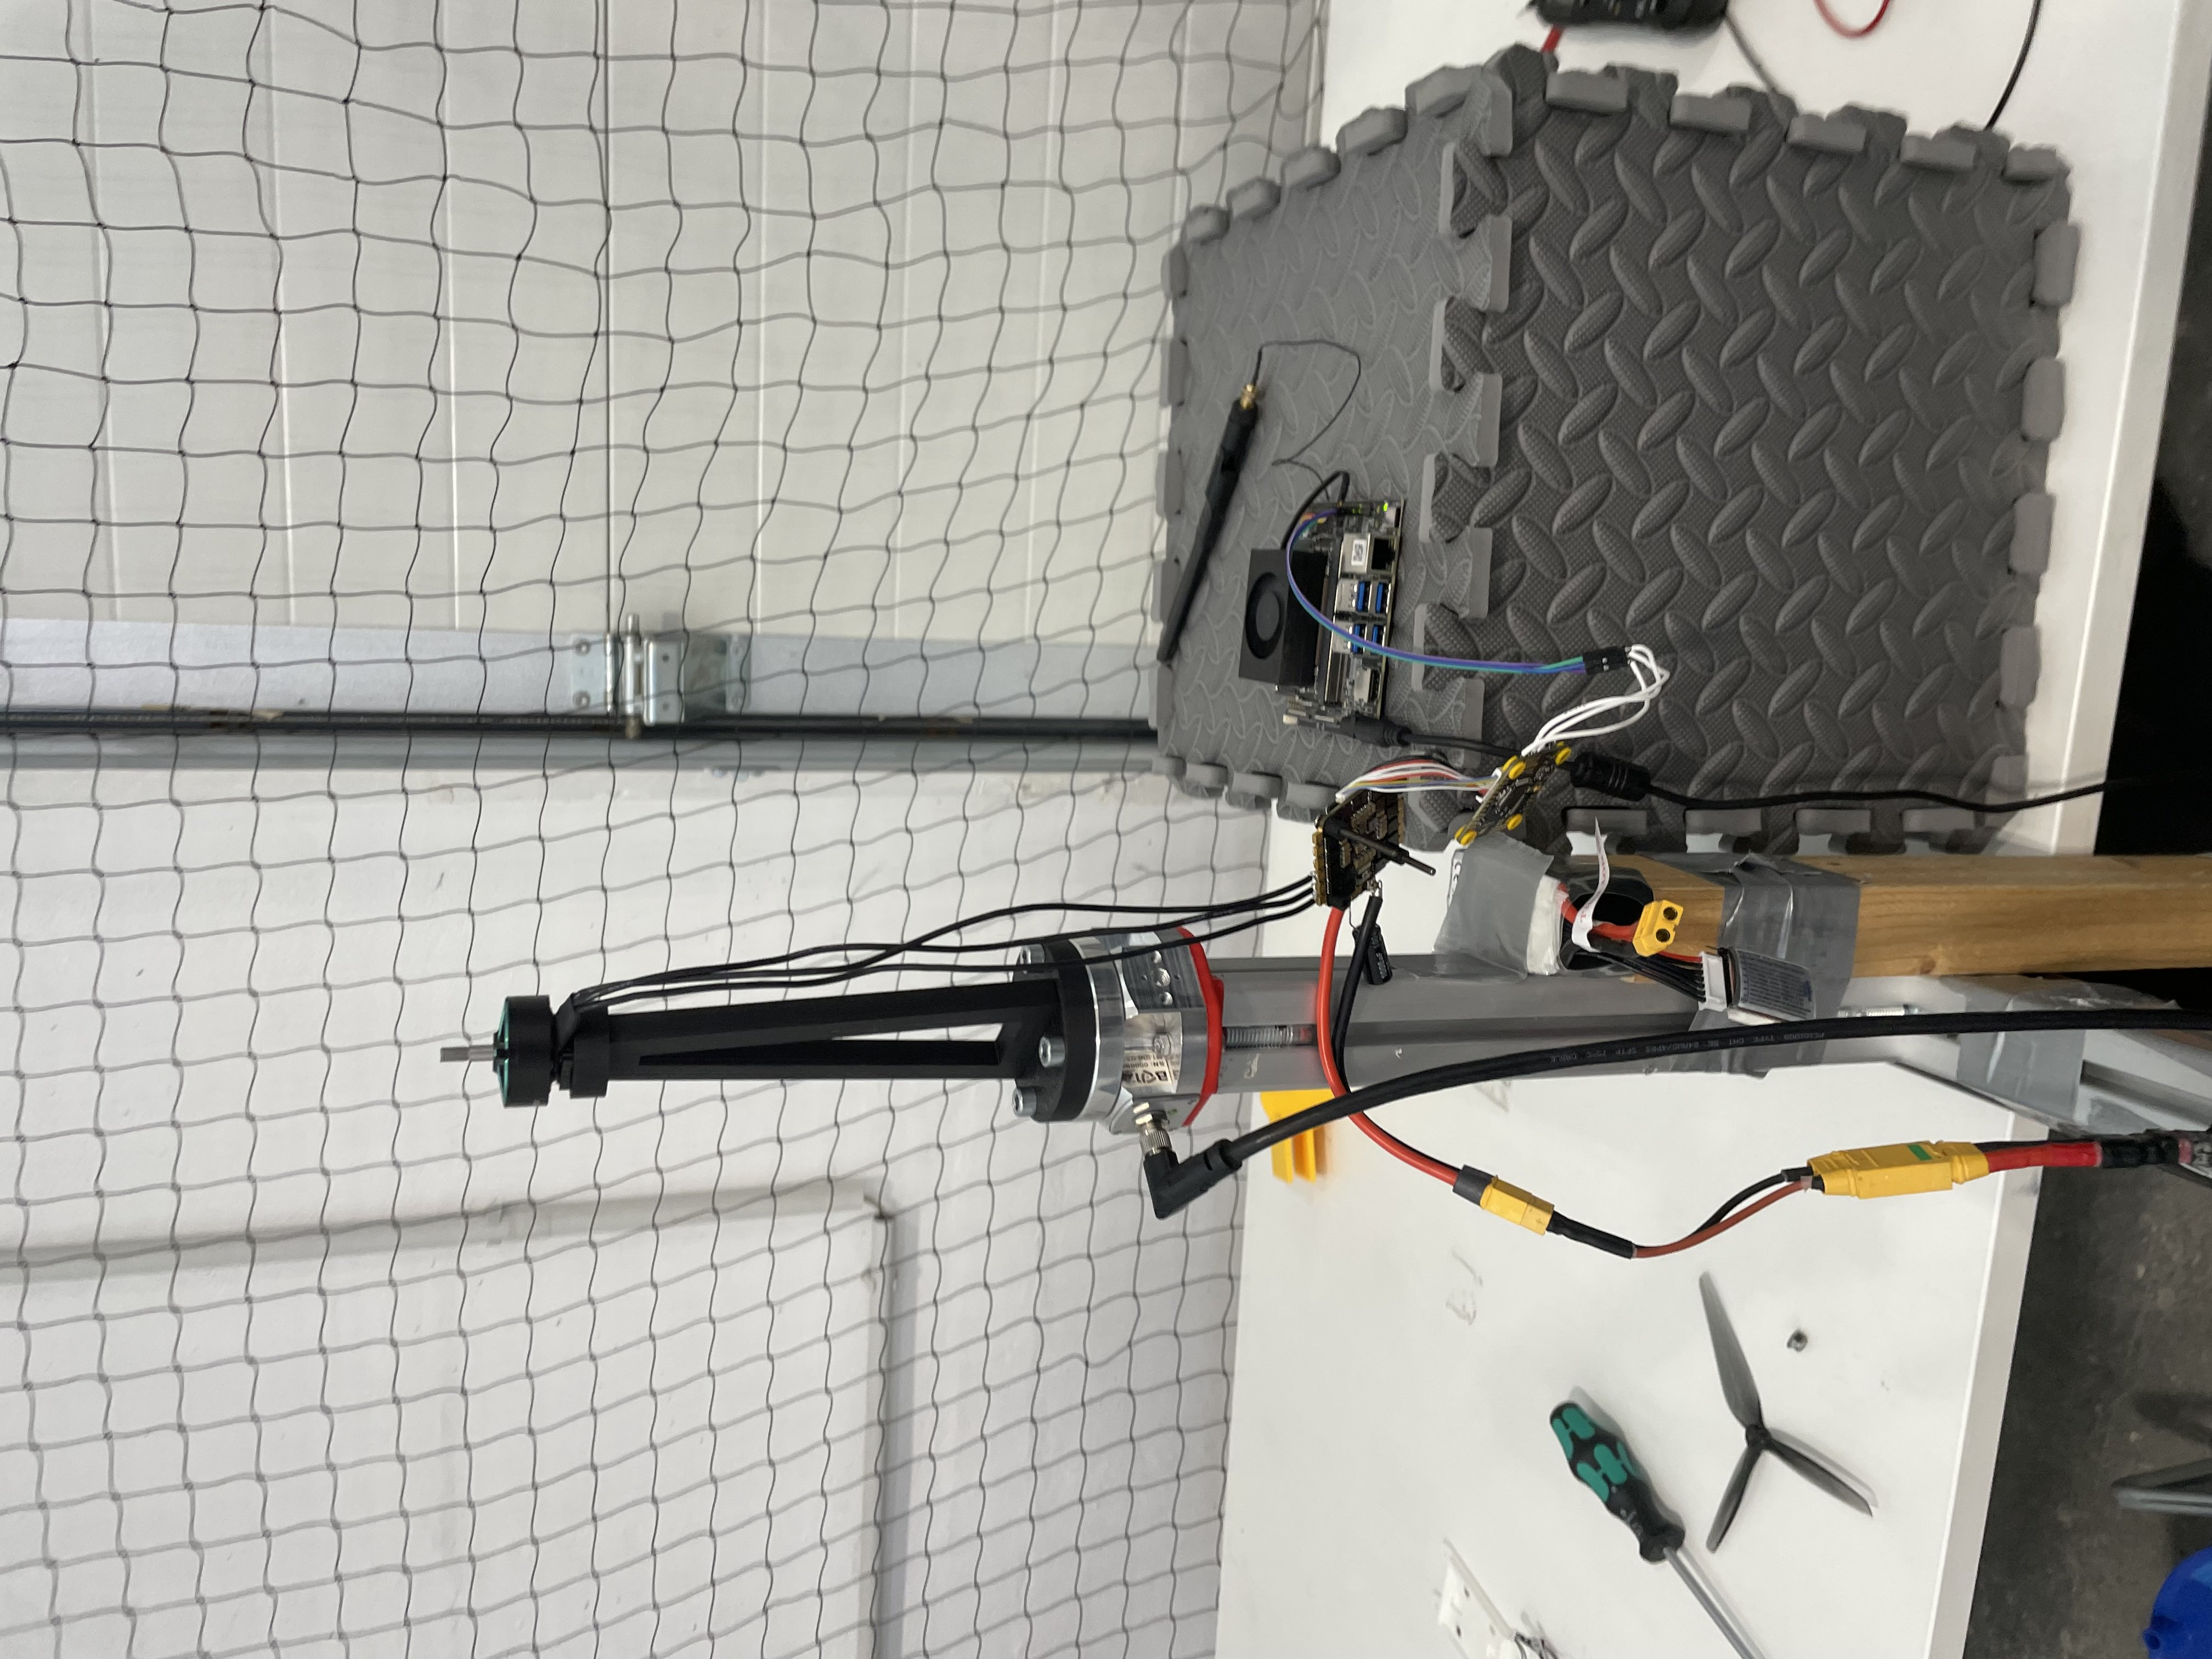
\includegraphics[width=0.85\linewidth,angle=-90]{figures/force_test_stand.jpg}};
\begin{scope}[x={(image.south east)},y={(image.north west)}]
    % Coordinates are relative: (0,0) = bottom-left, (1,1) = top-right
    % Adjust these coordinates to point to the correct components
    
    % Motor at the top
    \draw[->,thick,TUMBlue,line width=4pt] (0.5,0.85) -- (0.4,0.8);
    \node[TUMBlue,font=\normalsize,fill=white,fill opacity=0.85,text opacity=1,inner sep=5pt] at (0.5,0.9) {Motor};
    
    % Force sensor (Rokubi Mini - cylindrical part)
    \draw[->,thick,TUMBlue,line width=4pt] (0.2,0.35) -- (0.3,0.45);
    \node[TUMBlue,font=\normalsize,align=center,fill=white,fill opacity=0.85,text opacity=1,inner sep=5pt] at (0.2,0.3) {Rokubi Mini\\Force Sensor};
    
    % Battery (visible in lower portion)
    \draw[->,thick,TUMBlue,line width=4pt] (0.25,0.15) -- (0.35,0.2);
    \node[TUMBlue,font=\normalsize,fill=white,fill opacity=0.85,text opacity=1,inner sep=5pt] at (0.15,0.15) {Battery};

    % Jetson (visible in lower portion)
    \draw[->,thick,TUMBlue,line width=4pt] (0.75,0.6) -- (0.65,0.5);
    \node[TUMBlue,font=\normalsize,fill=white,fill opacity=0.85,text opacity=1,inner sep=5pt] at (0.75,0.65) {Jetson};

    % FC and ESC (visible in lower portion)
    \draw[->,thick,TUMBlue,line width=4pt] (0.7,0.2) -- (0.55,0.3);
    \node[TUMBlue,font=\normalsize,fill=white,fill opacity=0.85,text opacity=1,inner sep=5pt] at (0.7,0.2) {FC and ESC};
\end{scope}
\end{tikzpicture}
\caption{Static thrust characterization test stand with motor mounted on Rokubi~Mini force–torque sensor.}
\label{fig:force_test_stand}
\end{figure}

Motor command values were swept across the full throttle range in incremental steps, and the resulting thrust was recorded.  
Each command level was averaged over a \SI{2}{\second} window to mitigate transient effects.  
The measurements yielded a nonlinear but monotonic mapping between normalized command input $u \in [0,1]$ and thrust output $T$, which was fitted with a second-order polynomial of the form
\begin{equation}
T(u) = a_2 u^2 + a_1 u + a_0,
\end{equation}
where the coefficients $a_i$ were obtained via least-squares regression.

This empirical mapping was subsequently integrated into the control pipeline to convert desired thrust values from the INDI controller into per-motor DShot commands.  
The calibrated relationship improved the accuracy of total thrust estimation and allowed for energy-based efficiency analysis during flight tests.

\paragraph{Power configuration considerations.}
During the bench tests, one motor was mounted on the force sensor while the remaining four motors stayed on the vehicle and were kept fixed. We observed that the command-to-thrust relationship depends on how many motors are simultaneously powered from the battery due to load-dependent voltage sag and internal resistance effects. In particular, running only a single motor from a single 6S pack produced a slightly different mapping than powering all four motors from the flight-representative configuration with two 6S packs in parallel (6S~2P). Unless stated otherwise, the mapping used for control in flight was calibrated under the latter 6S~2P, four-motor-powered condition, and all subsequent thrust conversions refer to this configuration.

\subsubsection{Avionics and Electrical System}
The avionics stack is based on a \textit{Kakute~H7~v1.5} flight controller paired with a 4-in-1 ESC. Two \SI{1400}{\milli\ampere\hour} 6S~Tattu~R-Line batteries are connected in parallel to power the propulsion and avionics subsystems, resulting in an effective \SI{2800}{\milli\ampere\hour} capacity. The onboard computer, an NVIDIA~Jetson~Orin~Nano~(8\,GB), is powered independently from a \SI{1800}{\milli\ampere\hour} 4S~LiPo battery.

A custom-modified version of \textit{Betaflight} firmware was employed on the flight controller to extract motor RPM and battery voltage data from the DShot interface and stream them over MAVLink. This modification was necessary because the stock Betaflight implementation does not support publishing these telemetry values via MAVLink. The onboard IMU integrated into the Kakute~H7 was used for all experiments; no external IMUs were installed. Vicon markers were arranged asymmetrically to ensure unambiguous pose tracking.

\begin{table}[h]
\centering
\caption{Bill of Materials (BOM) for the experimental platform.}
\label{tab:bom}
\small
\begin{tabularx}{\textwidth}{ll>{\raggedright\arraybackslash}X}
\toprule
Category & Component & Model / Key Specs \\
\midrule
Airframe & Frame & X-wing center frame with carbon wing spars \\
Airframe & Wings & Four fixed wings (length 450\,mm, chord 250\,mm; NACA~0015 airfoil), orthogonal layout ($90^{\circ}$ between adjacent wings); skins: Bambu Lab PLA Aero; spars: 10\,mm OD carbon tubes; total projected horizontal area $S_\mathrm{t}\approx 0.318$\,m$^2$ \\
Propulsion & Motors ($\times$4) & T-MOTOR VELOX~V2808, max~22\,N each \\
Propulsion & Propellers ($\times$4) & HQProp 7\,×\,3.5\,×\,3, 3-blade racing propeller (7", light grey) \\
Avionics & FC+ESC & Kakute~H7~v1.5 Stack (4-in-1~ESC) \\
Power & Battery ($\times$2, parallel) & Tattu~R-Line~V5.0~6S~1400\,mAh~150C, XT60; effective 6S~2800\,mAh (parallel) \\
Companion & Computer & Jetson~Orin~Nano~8\,GB (Ubuntu~20.04) \\
Companion & Power & Tattu~R-Line~V3.0~4S~1800\,mAh~120C, XT60 \\
Motion Capture & Markers & Four 2\,cm markers arranged in an asymmetric constellation \\
\bottomrule
\end{tabularx}
\end{table}

\subsection{Software}

\subsubsection{Architecture and Communication}
The onboard software stack consists of \textit{ROS~1~Noetic} running on the Jetson companion. The geometric controller with inner and outer INDI (Incremental Nonlinear Dynamic Inversion) loops was implemented in ROS and executed on the companion, which sent individual motor speed commands directly to the flight controller over MAVLink via UART. The flight controller, in turn, only relayed the received motor commands to the ESCs while providing IMU, motor RPM, and battery telemetry back to the companion.

A ROS master node was hosted on a ground station computer, while the Jetson ran a ROS node for flight control and data logging. Communication between the two systems was established via Wi-Fi. The ground station handled trajectory loading, arming, and manual control interfaces. All experiment data, including position, velocity, attitude, thrust commands, and battery voltage, were logged in \textit{rosbag} format for offline analysis in Python.

\subsubsection{Estimation and Control}
The state estimation pipeline used the Vicon motion capture system to provide real-time position and attitude feedback to the controller. In some experiments, an onboard Extended Kalman Filter (EKF) fused IMU data for state estimation. The Vicon system and onboard IMU operated in a consistent right-handed coordinate convention (front–left–up), with roll about the $x$-axis, pitch about $y$, and yaw about $z$.

All flight maneuvers, including point-to-point transitions and trajectory tracking, were executed fully autonomously from predefined setpoints. No separate failsafe was implemented for Vicon loss, but trajectories could be manually stopped and the vehicle landed or disarmed from the base station.

\subsection{Facilities}

\subsubsection{Motion Capture Systems}
Two different Vicon systems were employed for data acquisition and feedback.  
The smaller test arena in Munich measured approximately \SI{7}{\meter} × \SI{8}{\meter} and was used primarily for agility experiments, such as \SI{3}{g} circle maneuvers.  
The larger \textit{AIDA Hall} at Reutlingen University provided a volume of about \SI{60}{\meter} × \SI{45}{\meter}, enabling steady forward-flight efficiency trials (see Fig.~\ref{fig:aida_hall}).  
Both systems operated at a sampling rate of \SI{200}{\hertz}.  
Vicon data were used both as ground truth and as feedback for the control loop.

\begin{figure}[h]
\centering
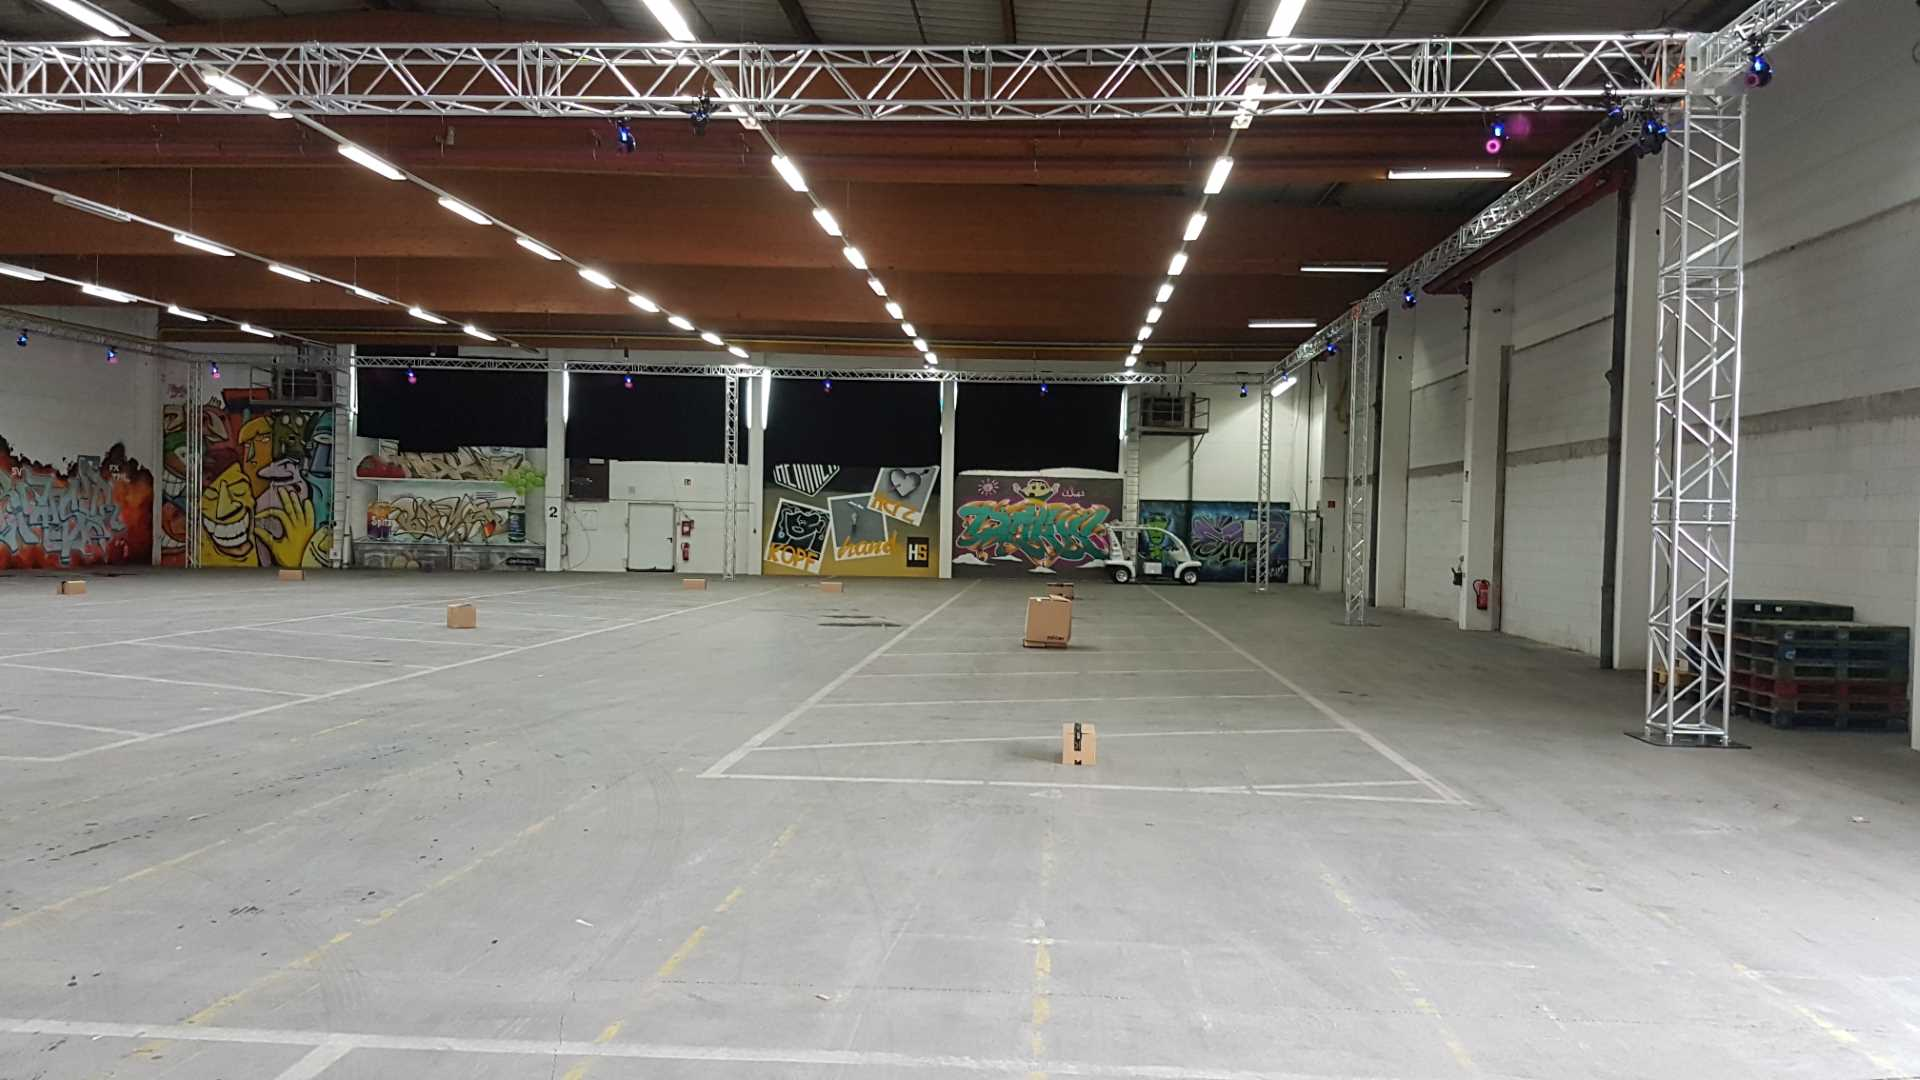
\includegraphics[width=0.85\linewidth]{figures/aida_hall.jpg}
\caption{AIDA Hall test facility used for efficiency trials (image credit: Reutlingen University~\cite{AIDAHallPhoto2024}).}
\label{fig:aida_hall}
\end{figure}

\subsubsection{Test Protocols}
Agility tests were performed in the Munich indoor arena equipped with safety nets and a soft landing surface.  
Efficiency tests were conducted in the AIDA Hall under still-air indoor conditions, with no wind sources or obstacles.  
Energy consumption was estimated from measured voltage, current draw, and propeller rotational speed data.  
Typical flight durations were approximately five minutes per run.

\subsubsection{Documentation}
All experiments were recorded through \textit{rosbag} logs and video footage to facilitate data visualization and reproducibility.  
Post-processing and analysis were conducted in Python, using custom scripts for trajectory evaluation, energy estimation, and control performance comparison.

% !TeX root = ../main.tex

\chapter{Experiments and Evaluation}\label{chapter:experiments-evaluation}

We design experiments to validate thrust mapping, agility/controllability, aerodynamic disturbance characterization, and efficiency gains.

\section{Thrust map identification}
Throttle-to-thrust and RPM-to-thrust mapping; present identified curves and fitted models.

\begin{figure}[htbp]
  \centering
  \begin{tikzpicture}
  \begin{axis}[tumplot, xlabel={RPM [rev/min]}, ylabel={Thrust [N]}, width=0.8\textwidth]
      % Original scatter data points
      \addplot[only marks, mark=*, mark size=1pt, opacity=0.5, TUMBlue]
        table[x=rpm_motor1, y=force_z_N, col sep=comma]{data/thrust_map_raw_data.csv};
      \addlegendentry{Measured data}
      % Quadratic fit curve
      \addplot[thick, TUMAccentOrange, no marks]
        table[x=rpm, y=thrust_N_fitted, col sep=comma]{data/thrust_vs_rpm_quadratic_fit.csv};
      \addlegendentry{Quadratic fit}
    \end{axis}
  \end{tikzpicture}
  \caption{Thrust vs RPM with quadratic fit: $T = 0.0515 \cdot \text{RPM}^2 - 0.0902 \cdot \text{RPM} - 0.996$ (N). $R^2 = 0.997$.}
  \label{fig:thrust_vs_rpm}
\end{figure}

\begin{figure}[htbp]
  \centering
  \begin{tikzpicture}
  \begin{axis}[tumplot, xlabel={Command [\%]}, ylabel={RPM [rev/min]}, width=0.8\textwidth]
      % Original scatter data points
      \addplot[only marks, mark=*, mark size=1pt, opacity=0.5, TUMBlue]
        table[x=cmd, y=rpm_motor1, col sep=comma]{data/thrust_map_raw_data.csv};
      \addlegendentry{Measured data}
      % Linear fit line
      \addplot[thick, TUMAccentOrange, no marks]
        table[x=cmd, y=rpm_fitted, col sep=comma]{data/rpm_vs_cmd_linear_fit.csv};
      \addlegendentry{Linear fit}
    \end{axis}
  \end{tikzpicture}
  \caption{RPM vs Command with linear fit: $\text{RPM} = 19.26 \cdot \text{cmd} + 3.65$ (rev/min). $R^2 = 0.991$.}
  \label{fig:rpm_vs_cmd}
\end{figure}

\begin{figure}[htbp]
  \centering
  \begin{tikzpicture}
  \begin{axis}[tumplot, xlabel={Command [-]}, ylabel={Thrust [N]}, width=0.8\textwidth]
      \addplot[only marks, mark=*, mark size=1pt, opacity=0.5, TUMBlue]
        table[x=cmd, y=force_z_N, col sep=comma]{data/thrust_vs_cmd_data.csv};
      \addlegendentry{Measured data}
    \end{axis}
  \end{tikzpicture}
  \caption{Thrust vs Command showing the direct relationship between motor command and thrust force.}
  \label{fig:thrust_vs_cmd}
\end{figure}

\section{Agility and tracking}
- 3g circles in flight arena; metrics: RMS position/attitude tracking error, control effort.

\section{Aerodynamic forces/moments quantification}
- Identify equivalent $k_D,k_L$ or $C_L(\alpha), C_D(\alpha)$ from maneuvering flight data; discuss sensitivity.

\section{Airfoil performance comparison and efficiency assessment}
\label{sec:airfoil_comparison}

\subsection{Aerodynamic characterization}

To evaluate the potential for improved efficiency through airfoil optimization, we analyzed two wing configurations using XFLR5: the baseline NACA~0015 symmetric airfoil and an improved AG25 profile.
The analysis covers Reynolds numbers of $Re=1\times10^5$, $Re=2\times10^5$, and $Re=5\times10^5$, representing the operational flight regime from low to moderate speeds.
The primary operational condition at \SI{10}{\meter\per\second} cruise speed corresponds to $Re=2\times10^5$.
All simulations use NCrit=5 to account for the free-stream turbulence typical of indoor and outdoor flight environments.

Figures~\ref{fig:cl_comparison}--\ref{fig:ld_comparison} present comprehensive aerodynamic comparisons at two Reynolds numbers ($Re=1\times10^5$ and $Re=5\times10^5$).
The results demonstrate excellent aerodynamic performance at operational Reynolds numbers, with the AG25 airfoil achieving lift-to-drag ratios exceeding 50 at low Reynolds numbers and above 60 at the cruise condition.

\begin{figure}[htbp]
\centering
% Reusable pgfplots styles for consistent thesis figures
\ProvidesFile{pgfplots_styles.tex}

% Base style for plots
\pgfplotsset{
  tumplot/.style={
    width=0.75\linewidth,
    height=0.45\linewidth,
    grid=both,
    thick,
    legend pos=south east,
    every axis plot/.append style={line join=round},
    % unify fonts with main text
    tick label style={font=\small},
    label style={font=\small},
    legend style={font=\small}
  },
  tumscatter/.style={only marks, mark size=1.7pt},
  tumorange/.style={color=TUMAccentOrange},
  tumgreen/.style={color=TUMAccentGreen},
  tumblue/.style={color=TUMBlue},
}

\begin{tikzpicture}
\begin{axis}[
  tumplot,
  width=0.85\textwidth,
  height=0.5\textwidth,
  xlabel={Angle of Attack, $\alpha$ [\si{\degree}]},
  ylabel={Lift Coefficient, $C_L$ [-]},
  legend pos=north west,
  grid=major,
]
\addplot[tumblue, thick] table[x=alpha, y=CL, col sep=comma] {scripts/data/CL_vs_alpha_NACA0015_Re0.100.csv};
\addlegendentry{NACA 0015, $Re=1\times10^5$}
\addplot[tumblue, thick, dashed] table[x=alpha, y=CL, col sep=comma] {scripts/data/CL_vs_alpha_NACA0015_Re0.500.csv};
\addlegendentry{NACA 0015, $Re=5\times10^5$}
\addplot[tumorange, thick] table[x=alpha, y=CL, col sep=comma] {scripts/data/CL_vs_alpha_AG25_Re0.100.csv};
\addlegendentry{AG25, $Re=1\times10^5$}
\addplot[tumorange, thick, dashed] table[x=alpha, y=CL, col sep=comma] {scripts/data/CL_vs_alpha_AG25_Re0.500.csv};
\addlegendentry{AG25, $Re=5\times10^5$}
\end{axis}
\end{tikzpicture}
\caption{Lift coefficient comparison between NACA~0015 and AG25 airfoils at two Reynolds numbers ($Re=1\times10^5$ and $Re=5\times10^5$), computed using XFLR5 with NCrit=5. At $Re=1\times10^5$, the AG25 achieves maximum \(C_L \approx 1.20\) at \SI{10}{\degree}, while the NACA~0015 reaches \(C_L \approx 0.97\) at \SI{12}{\degree}. Both airfoils show improved performance at higher Reynolds numbers, with more gradual stall characteristics and higher maximum lift coefficients.}
\label{fig:cl_comparison}
\end{figure}

\begin{figure}[htbp]
\centering
% Reusable pgfplots styles for consistent thesis figures
\ProvidesFile{pgfplots_styles.tex}

% Base style for plots
\pgfplotsset{
  tumplot/.style={
    width=0.75\linewidth,
    height=0.45\linewidth,
    grid=both,
    thick,
    legend pos=south east,
    every axis plot/.append style={line join=round},
    % unify fonts with main text
    tick label style={font=\small},
    label style={font=\small},
    legend style={font=\small}
  },
  tumscatter/.style={only marks, mark size=1.7pt},
  tumorange/.style={color=TUMAccentOrange},
  tumgreen/.style={color=TUMAccentGreen},
  tumblue/.style={color=TUMBlue},
}

\begin{tikzpicture}
\begin{axis}[
  tumplot,
  width=0.85\textwidth,
  height=0.5\textwidth,
  xlabel={Angle of Attack, $\alpha$ [\si{\degree}]},
  ylabel={Drag Coefficient, $C_D$ [-]},
  legend style={
    at={(0.5,1.0)},
    anchor=north
  },
  grid=major,
]
\addplot[tumblue, thick] table[x=alpha, y=CD, col sep=comma] {scripts/data/CD_vs_alpha_NACA0015_Re0.100.csv};
\addlegendentry{NACA 0015, $Re=1\times10^5$}
\addplot[tumblue, thick, dashed] table[x=alpha, y=CD, col sep=comma] {scripts/data/CD_vs_alpha_NACA0015_Re0.500.csv};
\addlegendentry{NACA 0015, $Re=5\times10^5$}
\addplot[tumorange, thick] table[x=alpha, y=CD, col sep=comma] {scripts/data/CD_vs_alpha_AG25_Re0.100.csv};
\addlegendentry{AG25, $Re=1\times10^5$}
\addplot[tumorange, thick, dashed] table[x=alpha, y=CD, col sep=comma] {scripts/data/CD_vs_alpha_AG25_Re0.500.csv};
\addlegendentry{AG25, $Re=5\times10^5$}
\end{axis}
\end{tikzpicture}
\caption{Drag coefficient comparison between NACA~0015 and AG25 airfoils at two Reynolds numbers. At $Re=1\times10^5$, the AG25 achieves minimum \(C_D \approx 0.011\) near \(\alpha = \SI{-1}{\degree}\), significantly lower than the NACA~0015's \(C_D \approx 0.015\) at \(\alpha = \SI{0}{\degree}\). The AG25 demonstrates superior low-drag characteristics across the operational angle of attack range, with drag coefficients approximately 25-30\% lower than the NACA~0015 baseline.}
\label{fig:cd_comparison}
\end{figure}

\begin{figure}[htbp]
\centering
% Reusable pgfplots styles for consistent thesis figures
\ProvidesFile{pgfplots_styles.tex}

% Base style for plots
\pgfplotsset{
  tumplot/.style={
    width=0.75\linewidth,
    height=0.45\linewidth,
    grid=both,
    thick,
    legend pos=south east,
    every axis plot/.append style={line join=round},
    % unify fonts with main text
    tick label style={font=\small},
    label style={font=\small},
    legend style={font=\small}
  },
  tumscatter/.style={only marks, mark size=1.7pt},
  tumorange/.style={color=TUMAccentOrange},
  tumgreen/.style={color=TUMAccentGreen},
  tumblue/.style={color=TUMBlue},
}

\begin{tikzpicture}
\begin{axis}[
  tumplot,
  width=0.85\textwidth,
  height=0.5\textwidth,
  xlabel={Drag Coefficient, $C_D$ [-]},
  ylabel={Lift Coefficient, $C_L$ [-]},
  legend style={
    at={(1.0,0.5)},
    anchor=east
  }
]
\addplot[tumblue, thick] table[x=CD, y=CL, col sep=comma] {scripts/data/drag_polar_NACA0015_Re0.100.csv};
\addlegendentry{NACA 0015, $Re=1\times10^5$}
\addplot[tumblue, thick, dashed] table[x=CD, y=CL, col sep=comma] {scripts/data/drag_polar_NACA0015_Re0.500.csv};
\addlegendentry{NACA 0015, $Re=5\times10^5$}
\addplot[tumorange, thick] table[x=CD, y=CL, col sep=comma] {scripts/data/drag_polar_AG25_Re0.100.csv};
\addlegendentry{AG25, $Re=1\times10^5$}
\addplot[tumorange, thick, dashed] table[x=CD, y=CL, col sep=comma] {scripts/data/drag_polar_AG25_Re0.500.csv};
\addlegendentry{AG25, $Re=5\times10^5$}
\end{axis}
\end{tikzpicture}
\caption{Drag polar comparison showing the relationship between lift and drag coefficients. Curves shifted toward the left and top indicate better aerodynamic efficiency (higher lift for given drag). At both Reynolds numbers, the AG25 demonstrates dramatically superior efficiency with the drag polar shifted significantly leftward compared to NACA~0015, achieving higher lift coefficients at substantially lower drag penalties. This improved polar translates directly to extended flight endurance and reduced power consumption.}
\label{fig:drag_polar}
\end{figure}

\begin{figure}[htbp]
\centering
% Reusable pgfplots styles for consistent thesis figures
\ProvidesFile{pgfplots_styles.tex}

% Base style for plots
\pgfplotsset{
  tumplot/.style={
    width=0.75\linewidth,
    height=0.45\linewidth,
    grid=both,
    thick,
    legend pos=south east,
    every axis plot/.append style={line join=round},
    % unify fonts with main text
    tick label style={font=\small},
    label style={font=\small},
    legend style={font=\small}
  },
  tumscatter/.style={only marks, mark size=1.7pt},
  tumorange/.style={color=TUMAccentOrange},
  tumgreen/.style={color=TUMAccentGreen},
  tumblue/.style={color=TUMBlue},
}

\begin{tikzpicture}
\begin{axis}[
  tumplot,
  width=0.85\textwidth,
  height=0.5\textwidth,
  xlabel={Angle of Attack, $\alpha$ [\si{\degree}]},
  ylabel={Lift-to-Drag Ratio, $L/D$ [-]},
  legend pos=south east,
  grid=major,
]
\addplot[tumblue, thick] table[x=alpha, y=LD, col sep=comma] {scripts/data/LD_vs_alpha_NACA0015_Re0.100.csv};
\addlegendentry{NACA 0015, $Re=1\times10^5$}
\addplot[tumblue, thick, dashed] table[x=alpha, y=LD, col sep=comma] {scripts/data/LD_vs_alpha_NACA0015_Re0.500.csv};
\addlegendentry{NACA 0015, $Re=5\times10^5$}
\addplot[tumorange, thick] table[x=alpha, y=LD, col sep=comma] {scripts/data/LD_vs_alpha_AG25_Re0.100.csv};
\addlegendentry{AG25, $Re=1\times10^5$}
\addplot[tumorange, thick, dashed] table[x=alpha, y=LD, col sep=comma] {scripts/data/LD_vs_alpha_AG25_Re0.500.csv};
\addlegendentry{AG25, $Re=5\times10^5$}
\end{axis}
\end{tikzpicture}
\caption{Lift-to-drag ratio comparison highlighting the aerodynamic efficiency of both airfoils. At $Re=1\times10^5$, the AG25 achieves a remarkable maximum L/D of 53.0 at $\alpha \approx \SI{5}{\degree}$, with L/D ratios exceeding 50 between \SI{4}{\degree} and \SI{6}{\degree}—substantially higher than the NACA~0015's maximum L/D of 37.1 at \SI{6}{\degree}. At typical cruise angles (\SI{4}{\degree}--\SI{6}{\degree}), the AG25 maintains L/D ratios above 50, representing a 30--43\% improvement over the NACA~0015 baseline and enabling significantly more efficient forward flight.}
\label{fig:ld_comparison}
\end{figure}

\paragraph{Key aerodynamic findings.}
Table~\ref{tab:airfoil_metrics} summarizes the key performance metrics for both airfoils at $Re=2\times10^5$, which corresponds to the typical cruise speed of \SI{10}{\meter\per\second}.

\begin{table}[htbp]
\centering
\caption{Aerodynamic performance metrics comparison at $Re=2\times10^5$ (NCrit=5).}
\label{tab:airfoil_metrics}
\begin{tabular}{lcc}
\hline
\textbf{Metric} & \textbf{NACA 0015} & \textbf{AG25} \\
\hline
Maximum $L/D$ & 46.4 at \SI{7}{\degree} & 66.4 at \SI{5}{\degree} \\
$C_L$ at max $L/D$ & 0.81 & 0.83 \\
$C_D$ at max $L/D$ & 0.018 & 0.013 \\
Minimum $C_D$ & 0.010 at \SI{0}{\degree} & 0.008 at \SI{0}{\degree} \\
Maximum $C_L$ & 1.05 at \SI{13}{\degree} & 1.27 at \SI{11}{\degree} \\
$L/D$ at \SI{4}{\degree} cruise & 34.3 & 66.2 \\
$L/D$ at \SI{6}{\degree} cruise & 43.9 & 64.4 \\
\hline
\end{tabular}
\end{table}

The AG25 airfoil demonstrates a 43\% improvement in maximum lift-to-drag ratio compared to the NACA~0015 (66.4 vs 46.4), achieved at a lower angle of attack (\SI{5}{\degree} vs \SI{7}{\degree}).
At typical cruise conditions between \SI{4}{\degree} and \SI{6}{\degree}, the AG25 maintains exceptional L/D ratios of 64--66, representing a 47--93\% improvement over the NACA~0015 baseline.
The AG25 also achieves 20\% lower minimum drag coefficient (0.008 vs 0.010) and 21\% higher maximum lift coefficient (1.27 vs 1.05).
Most notably, at the \SI{4}{\degree} cruise condition, the AG25 achieves L/D = 66.2, nearly double the NACA~0015's L/D = 34.3, translating directly to approximately 50\% reduction in required aerodynamic power for the same flight speed.
This substantial efficiency advantage across the entire operational envelope motivated the development of an improved platform variant incorporating the AG25 airfoil for efficiency-focused flight tests.

\subsection{Flight test efficiency comparison}

To validate the predicted aerodynamic improvements, we conducted comparative flight tests using both the baseline NACA~0015 platform (\SI{2.5}{\kg}) and the improved AG25 platform (\SI{2.2}{\kg}).

% TODO: Add power consumption comparison plots from flight data
% TODO: Add specific energy consumption (Wh/km) or endurance comparison
% TODO: Discuss correlation between predicted L/D improvement and measured efficiency gains

\subsection{Efficiency assessment summary}
- Compare theoretical quad thrust input vs. measured thrust input in AIDA hall flights; quantify energy savings due to passive lift.

\section{Baseline comparison}
- Compare against baseline quadrotor controller without INDI or without wings.

% !TeX root = ../main.tex

\chapter{Conclusion}\label{chapter:conclusion}

We summarize contributions: design of an aerodynamic surface-enhanced quadrotor, a robust INDI-based tracking controller, and experimental validation demonstrating accurate agile tracking and improved forward-flight efficiency. We outline future work, including refined aerodynamic modeling, coordinated-turn guidance integration, and extended outdoor testing.


\appendix{}

\microtypesetup{protrusion=false}

\addchap{Abbreviations}
\begin{acronym}
	\itemsep-.25\baselineskip
	\acro{UAV}[UAV]{Unmanned Aerial Vehicle}
	\acro{MAV}[MAV]{Micro Air Vehicle}
	\acro{VTOL}[VTOL]{Vertical Take-Off and Landing}
	\acro{INDI}[INDI]{Incremental Nonlinear Dynamic Inversion}
	\acro{EoM}[EoM]{Equations of Motion}
	\acro{DoF}[DoF]{Degrees of Freedom}
	\acro{CoG}[CoG]{Center of Gravity}
	\acro{CoP}[CoP]{Center of Pressure}
	\acro{IMU}[IMU]{Inertial Measurement Unit}
	\acro{Vicon}[Vicon]{Vicon Motion Capture System}
	\acro{FC}[FC]{Flight Controller}
	\acro{ESC}[ESC]{Electronic Speed Controller}
	\acro{RPM}[RPM]{Revolutions per Minute}
	% TODO: add acronyms
\end{acronym}

\listoffigures{}
\listoftables{}
\microtypesetup{protrusion=true}
\printbibliography{}

\end{document}
